\chapter{三维光场人脸光照编辑技术基础}
光场技术能够同时记录光线“从哪里来、朝哪里去”，因此相比传统二维图像更适合表达真实三维场景。围绕这一能力，三维光场人脸光照编辑的目标可概括为：在跨视角一致与时间连续的前提下，重建并重塑人脸在复杂照明下的外观变化。本章从基础理论出发，对后续方法所需的关键知识进行重组，包括立体视觉感知机制、光场显示实现路径、光照与渲染物理模型以及定量评价体系。具体而言，先讨论人眼如何利用深度线索形成空间知觉，再介绍基于光栅的裸眼 3D 光场显示流程；随后梳理相机成像、球谐光照、传统渲染与 NeRF 体渲染等核心建模方法；最后给出 PSNR、SSIM、FID、LPIPS 等客观指标及其使用场景。与常规图像编辑任务不同，光场人脸光照编辑不仅要求单帧“看起来像”，还要求在视点切换时保持身份、几何和阴影逻辑不跳变，因此本章在组织上强调“感知机制—显示实现—物理建模—评价闭环”的递进关系。通过这种编排方式，后续章节可直接复用本章术语体系与评价口径，减少方法描述中的重复定义。同时，这种先理论后实现、先模型后评价的组织方式也便于读者在阅读实验章节时快速回溯到对应基础。上述内容共同构成本文第二章的理论底座。
\section{三维光场显示原理}
现有消费级显示设备大多仍停留在二维成像层面，空间深度需要依赖额外编码才能被观察者正确感知。人眼之所以能够“看出前后层次”，本质上是多种线索共同作用的结果。为便于分析，本文将其归纳为两组：一类是经验驱动的心理线索，另一类是由眼球结构与神经处理直接产生的生理线索。二者并非互斥关系，而是在观看过程中持续融合：当前景和背景纹理给出粗粒度深度判断时，双目系统会进一步给出更精细的距离修正；当显示系统参数不匹配时，心理线索与生理线索甚至可能出现冲突，从而引发观看疲劳。
\subsection{立体视觉原理}
(1)心理反应因素

在真实观看环境中，心理线索往往先于生理线索起作用：观察者会先根据画面构图和经验判断大致空间布局，再通过眼动与双目机制完成细节确认。因此，面向光场内容生产时，除了保证几何正确，还需要关注构图连贯、主体突出和阴影一致等“可读性”因素。

纹理梯度：如图\ref{fig:2-1}(a)所示，纹理单元沿深度方向的疏密变化会被视觉系统解释为距离变化，从而帮助观察者快速建立前后层级\cite{Gibson1950}。

透视关系：图\ref{fig:2-1}(b)对应经典透视规律。随着距离增加，目标在成像平面上的投影会按比例缩小，这一几何关系是二维画面传递纵深感的核心线索\cite{Kaufman2000}。

阴影分布：图\ref{fig:2-1}(c)显示，阴影轮廓和亮度过渡同时反映了光照方向与几何起伏。借助这些线索，观察者可以在单幅图像中推断局部凹凸关系\cite{Shafer1985}。
\begin{figure}[H]
  \centering
  % 第一张子图（左侧）
  \begin{minipage}{0.32\textwidth}  % 3张子图均分宽度，0.32*3≈0.96，留少量间距
    \centering
    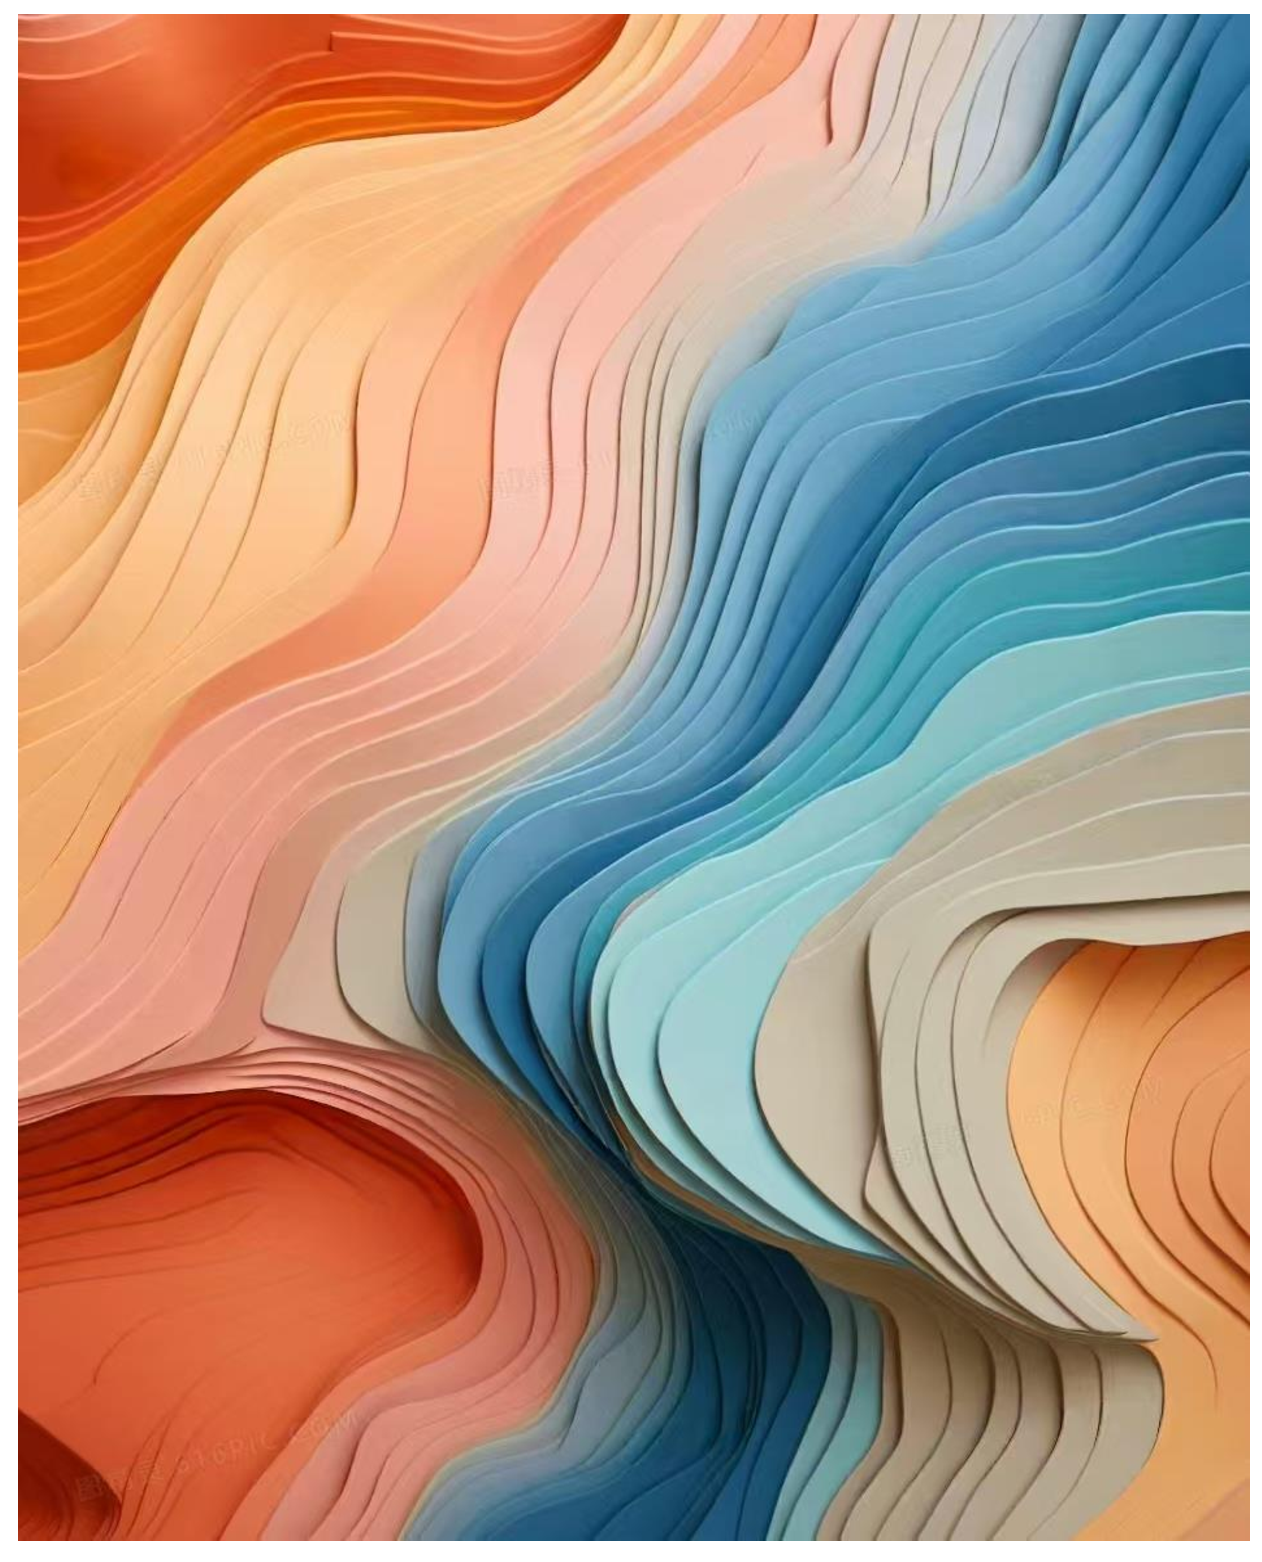
\includegraphics[width=0.9\linewidth, height=3.5cm]{resources/2p/2-1a.pdf}
    \centering\small(a)
    \label{fig:2-1a}
  \end{minipage}
  \hfill  % 子图间水平间距，自动均分空白
  % 第二张子图（中间）
  \begin{minipage}{0.32\textwidth}
    \centering
    
\includegraphics[width=0.9\linewidth, height=3.5cm]{resources/2p/2-1b.pdf}
    \centering\small(b)
    \label{fig:2-1b}
  \end{minipage}
  \hfill
  % 第三张子图（右侧）
  \begin{minipage}{0.32\textwidth}
    \centering
    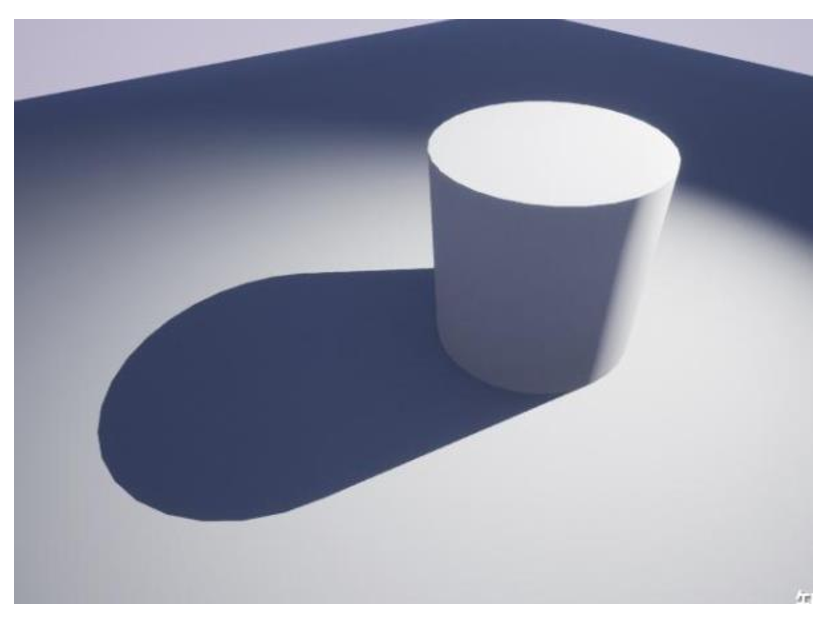
\includegraphics[width=0.9\linewidth, height=3.5cm]{resources/2p/2-1c.pdf}  % 替换为你的第三张图路径
    \centering\small(c)
    \label{fig:2-1c}
  \end{minipage}
  % 大图标题：补充第三张子图说明
  \caption{ (a)纹理示意图 (b)透视关系示意图 (c)阴影示意图}  % 替换XXX为你的第三张图说明
  \label{fig:2-1}
\end{figure}
(2)生理反应因素

与上述心理线索不同，生理线索由眼球成像与眼动控制直接产生，其中最关键的是双目视差\cite{Howard2002}。这也是三维显示系统设置视差与观看区参数时必须遵循的生物学基础\cite{Atchison2005}，如图\ref{fig:2-2}所示。

\begin{figure}[htbp]
  \centering
  % 第一张子图
  \begin{minipage}{0.49\textwidth}
    \centering
    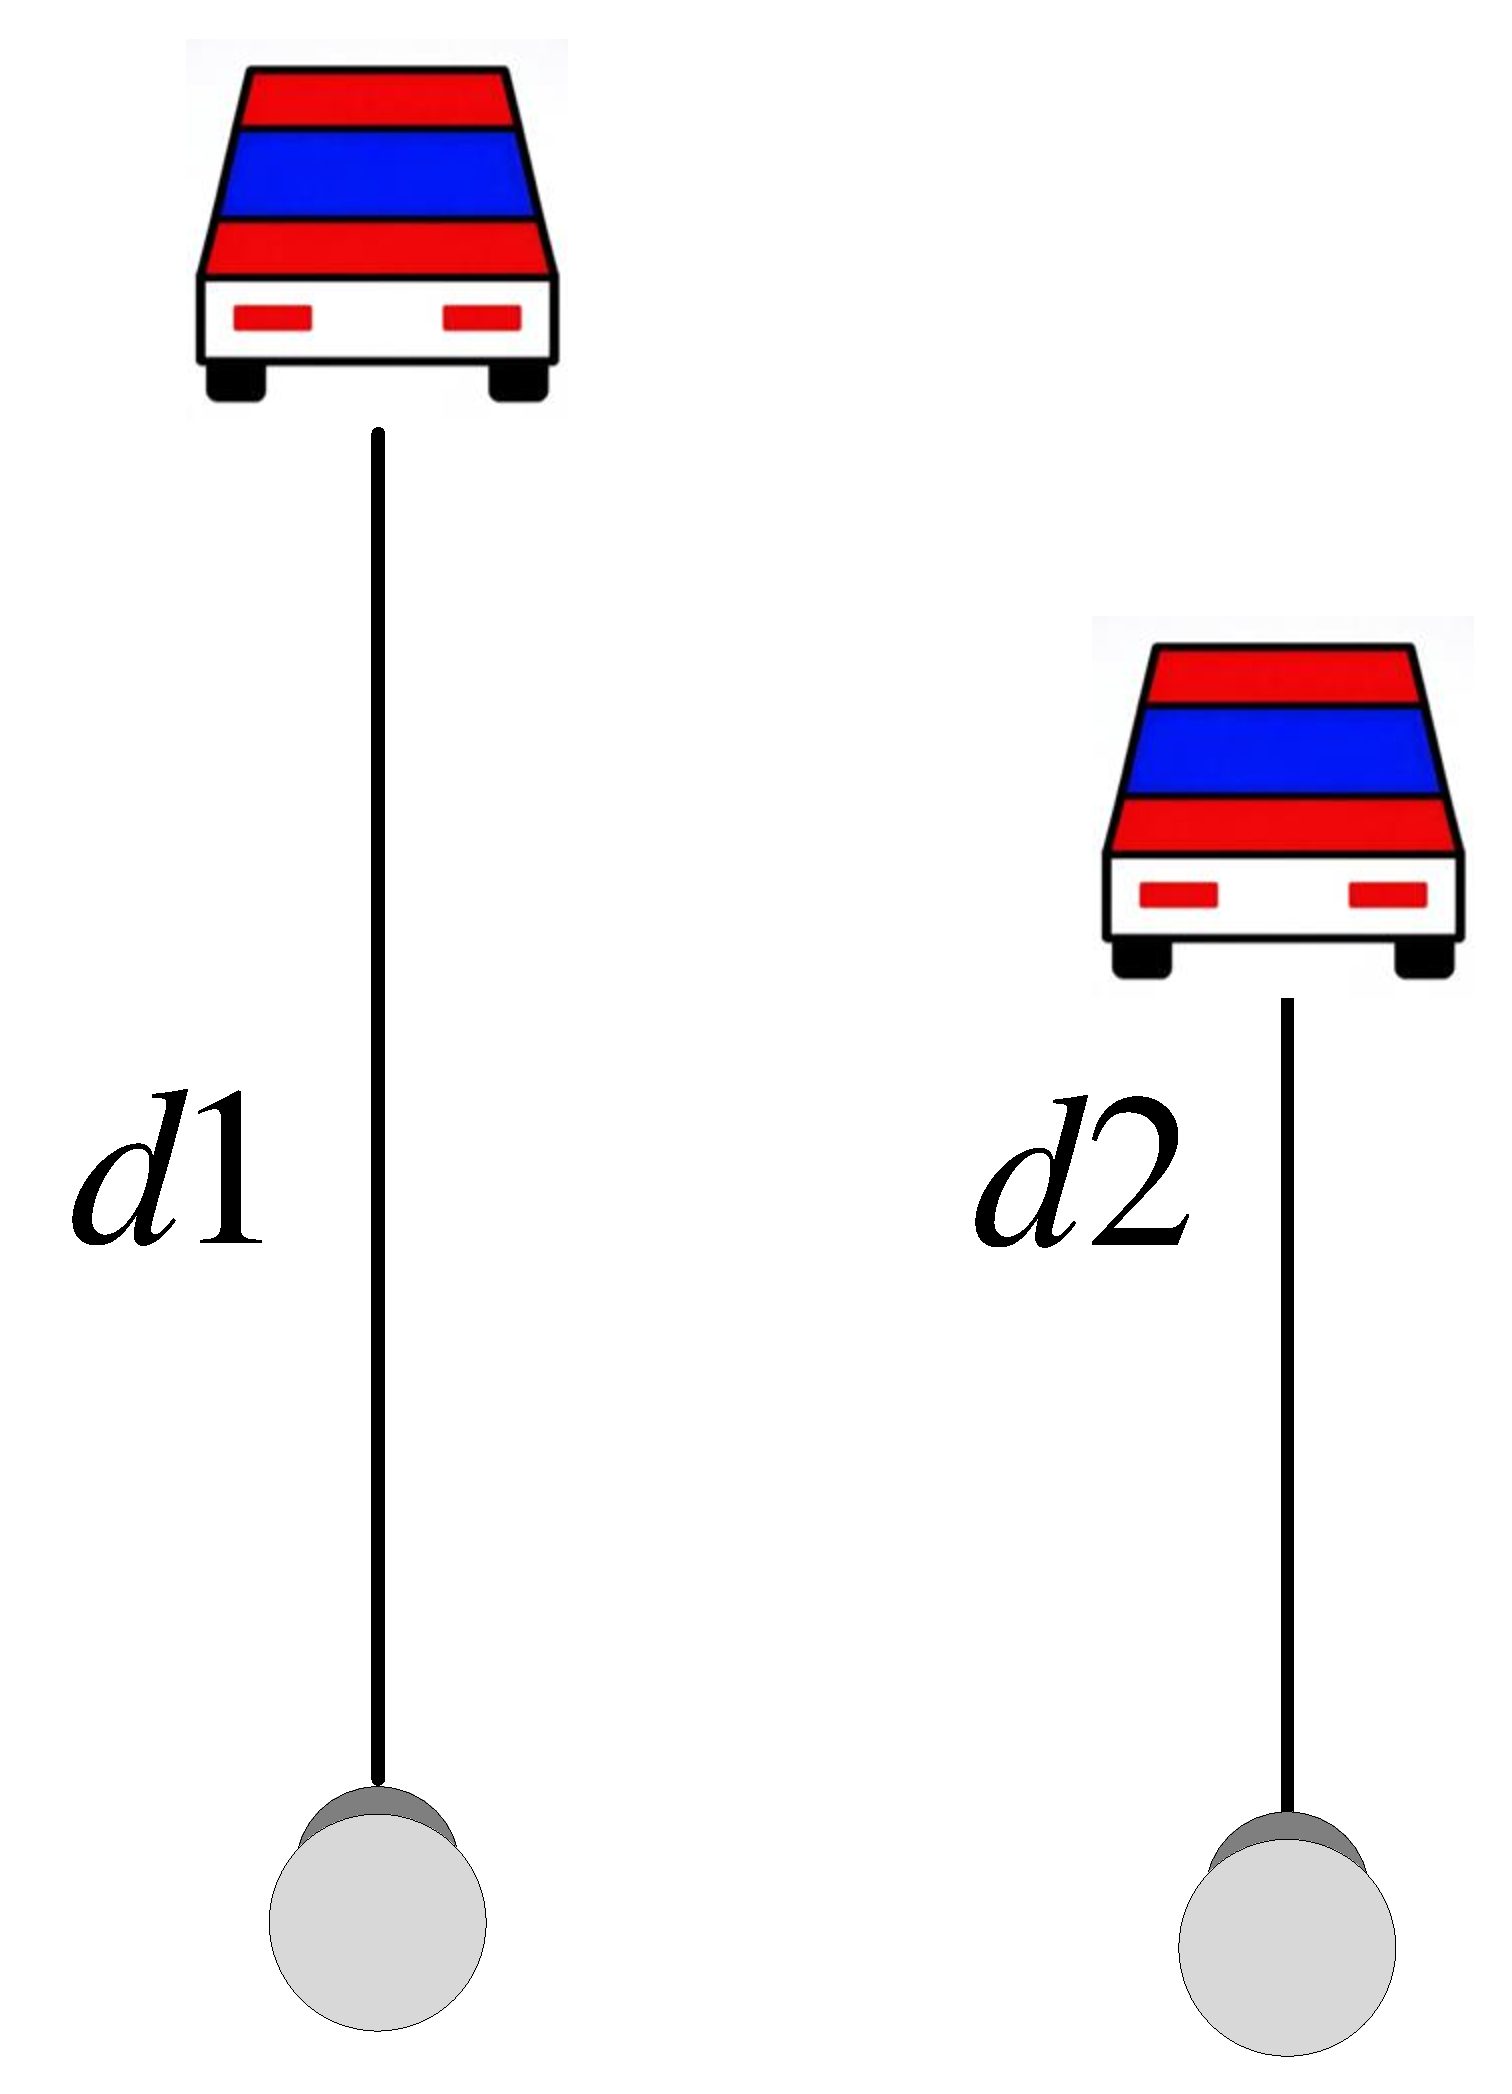
\includegraphics[width=0.8\linewidth, height=4cm]{resources/2p/2-2a.pdf}
    
    \centering\small(a)
    \label{fig:1-1a}
  \end{minipage}
  \hfill
  % 第二张子图
  \begin{minipage}{0.49\textwidth}
    \centering
    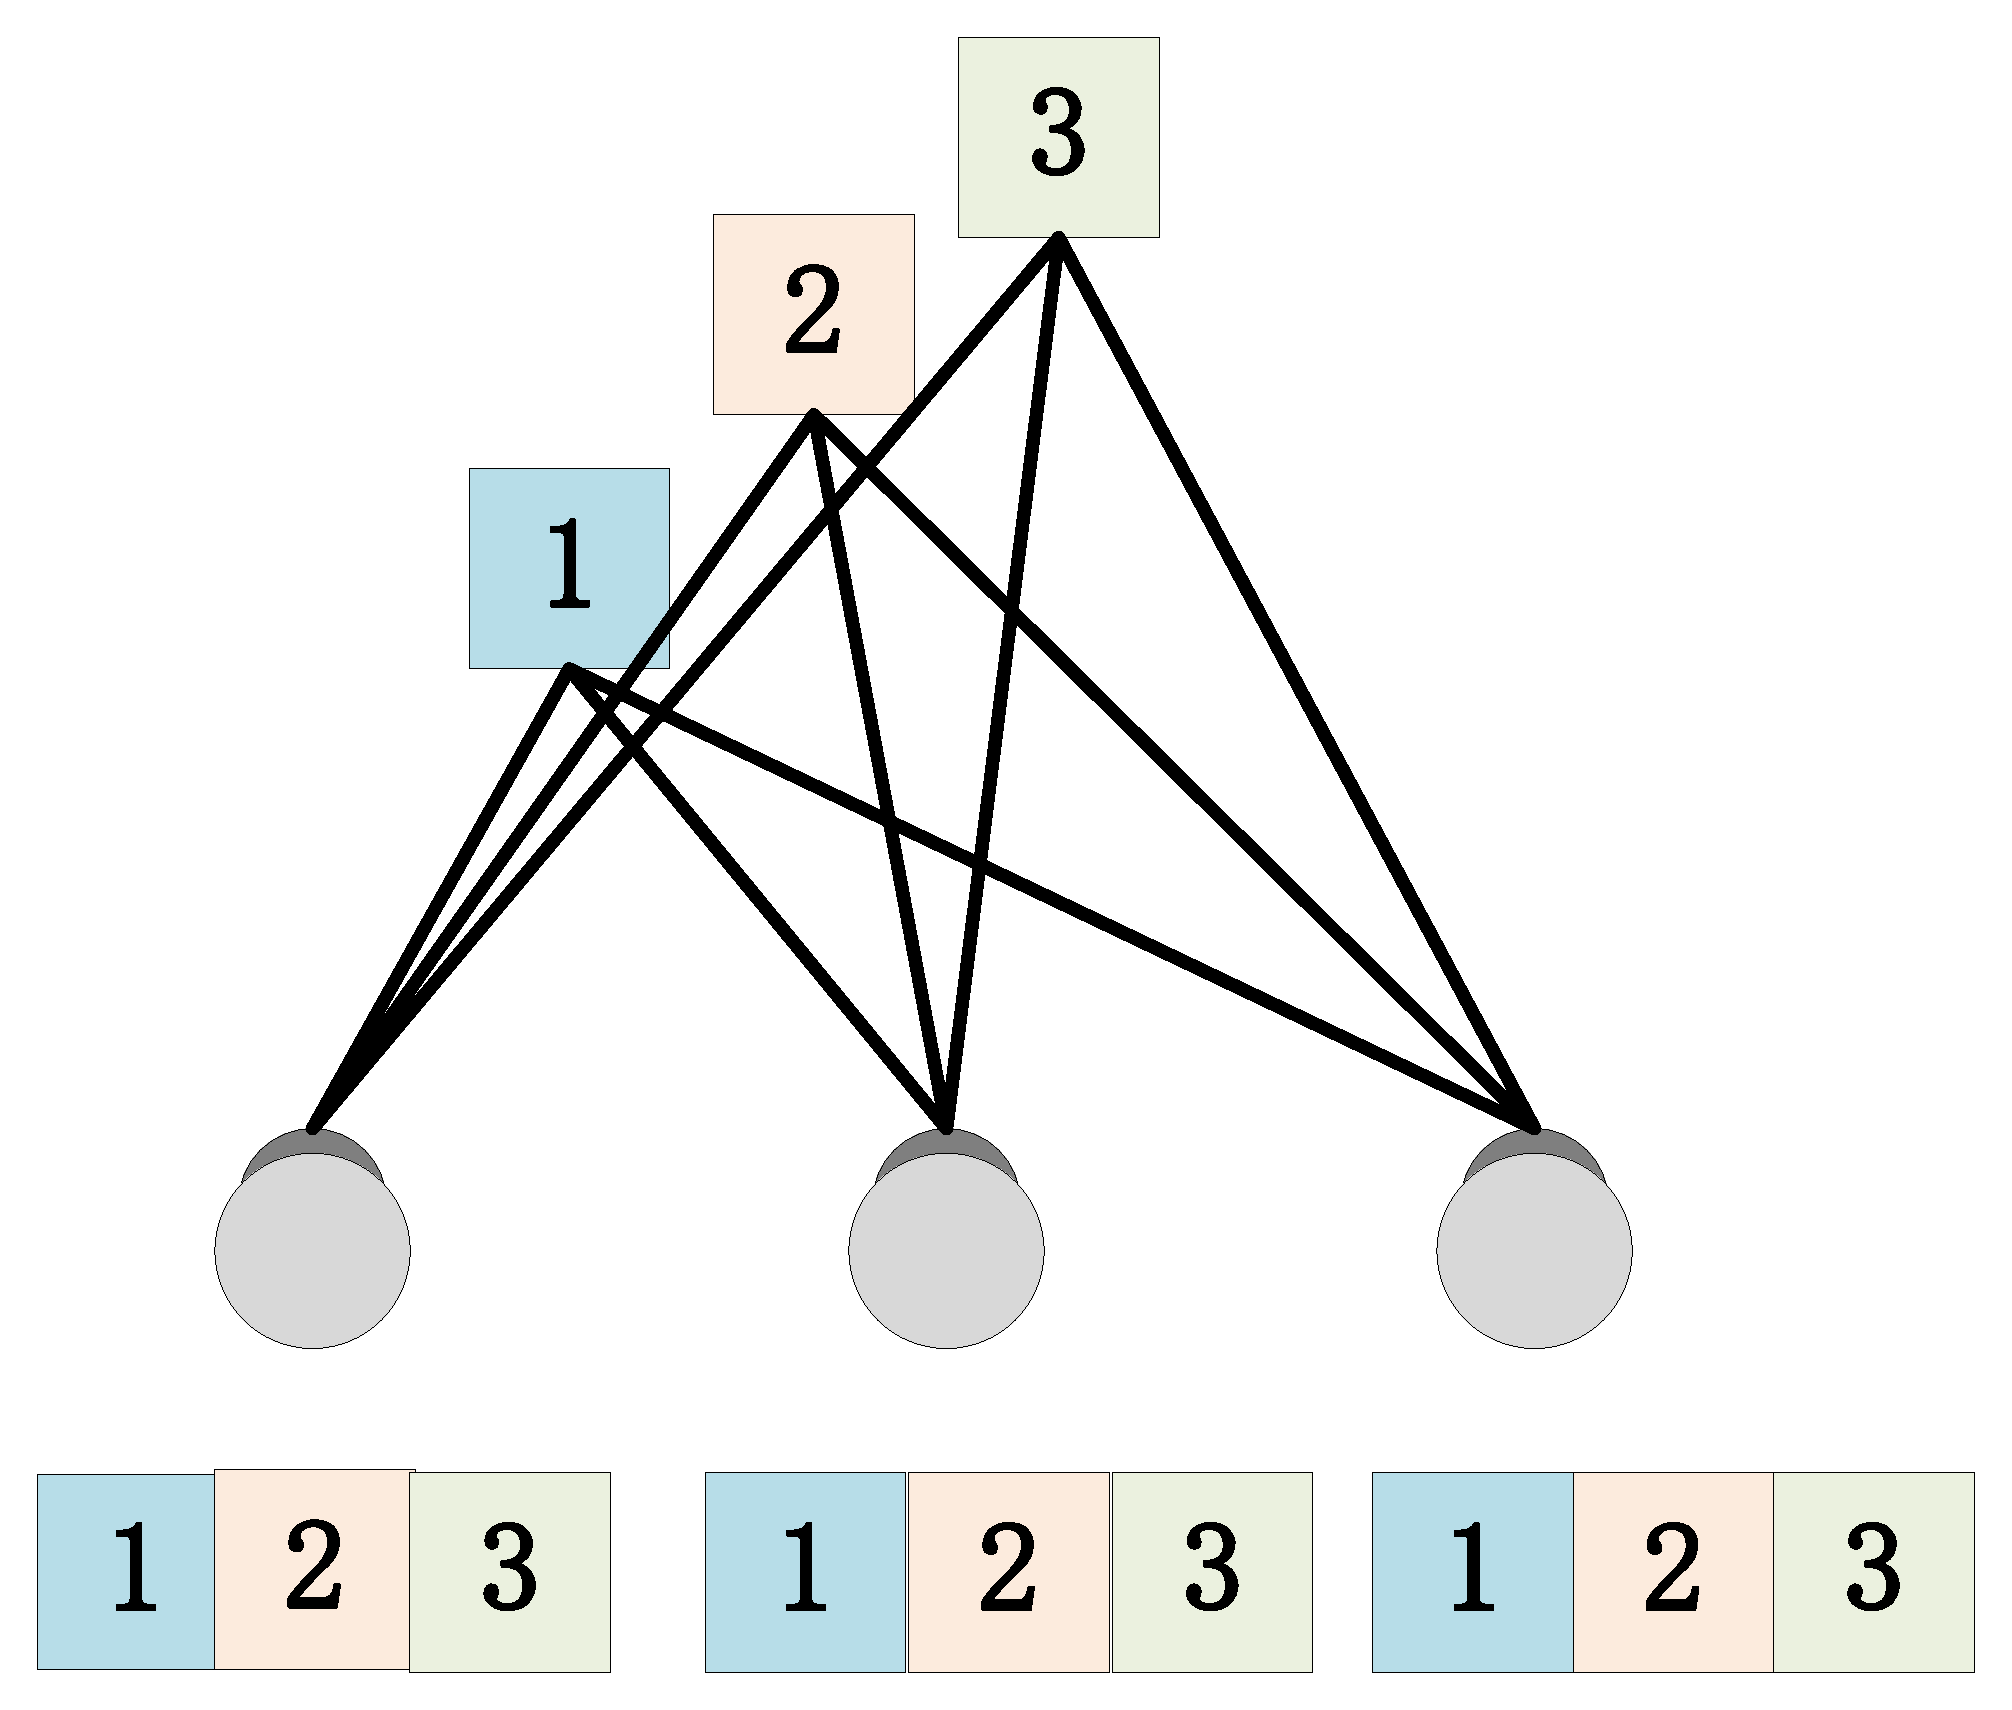
\includegraphics[width=0.9\linewidth, height=4cm]{resources/2p/2-2b.pdf}
    
    \centering\small(b)
    \label{fig:1-1b}
  \end{minipage}

  \vspace{0.5cm}

  % 第三张子图
  \begin{minipage}{0.49\textwidth}
    \centering
    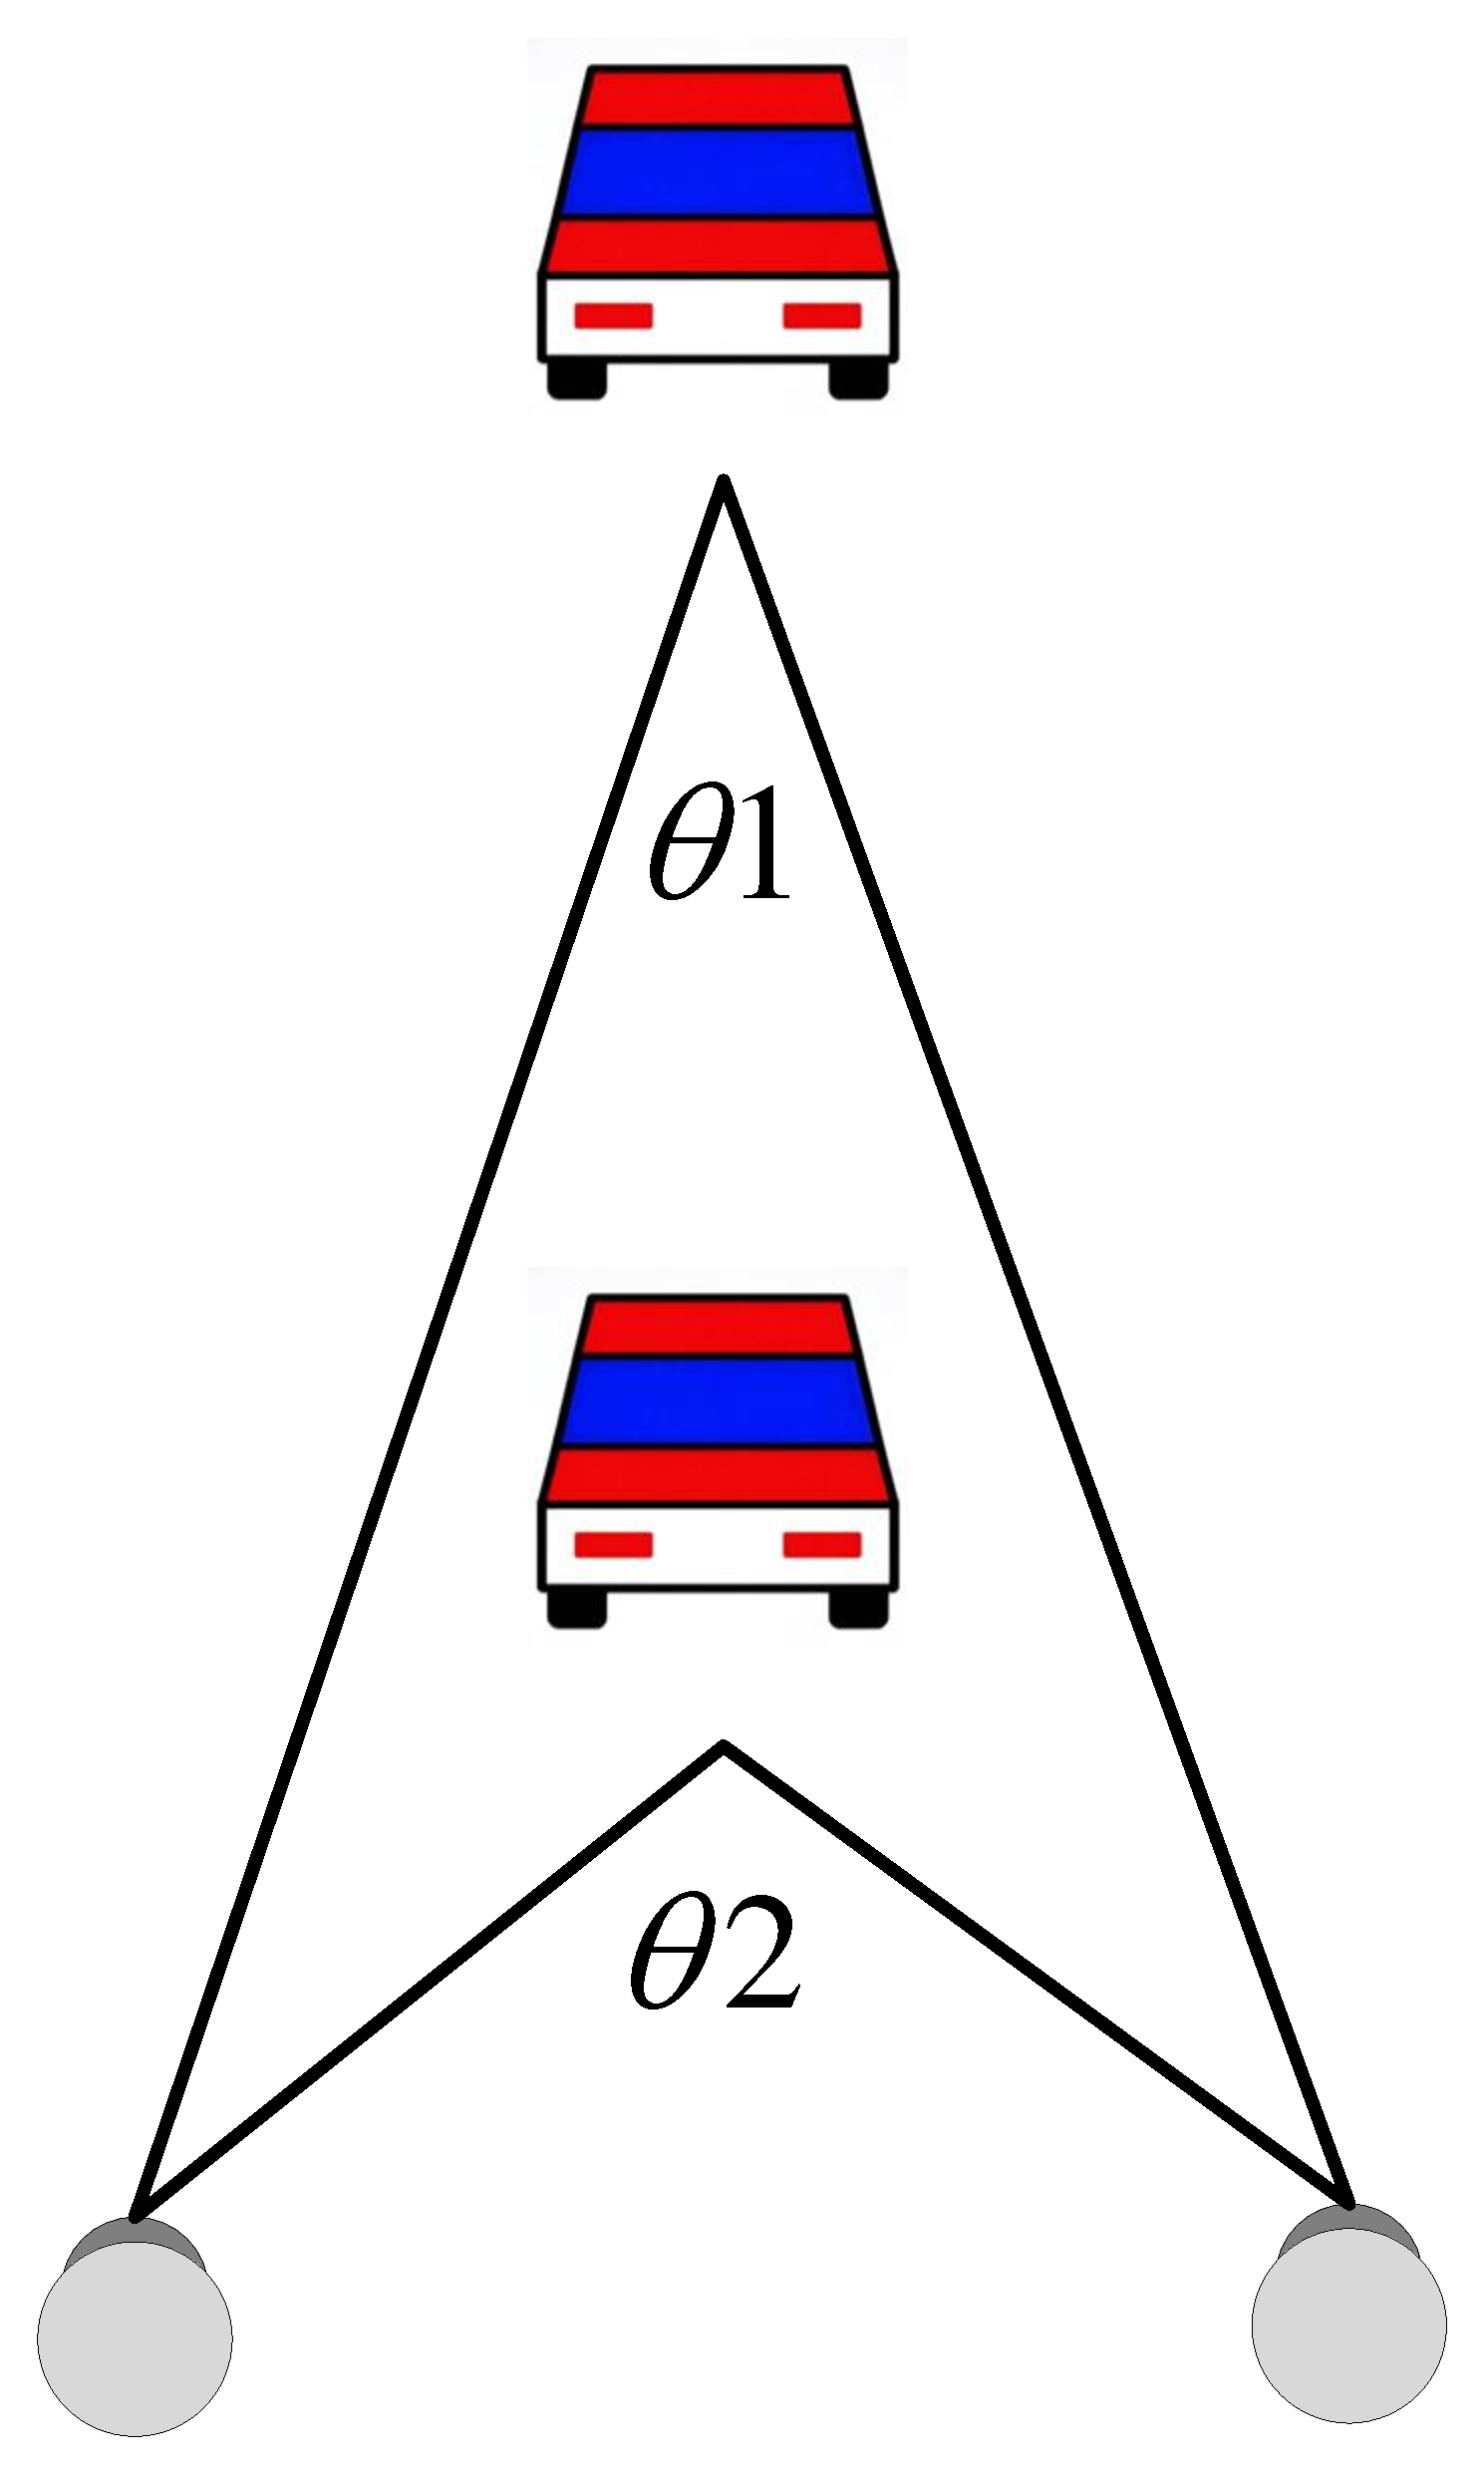
\includegraphics[width=0.8\linewidth, height=4cm]{resources/2p/2-2c.pdf}
    
    \centering\small(c) 
    \label{fig:1-1c}
  \end{minipage}
  \hfill
  % 第四张子图
  \begin{minipage}{0.49\textwidth}
    \centering
    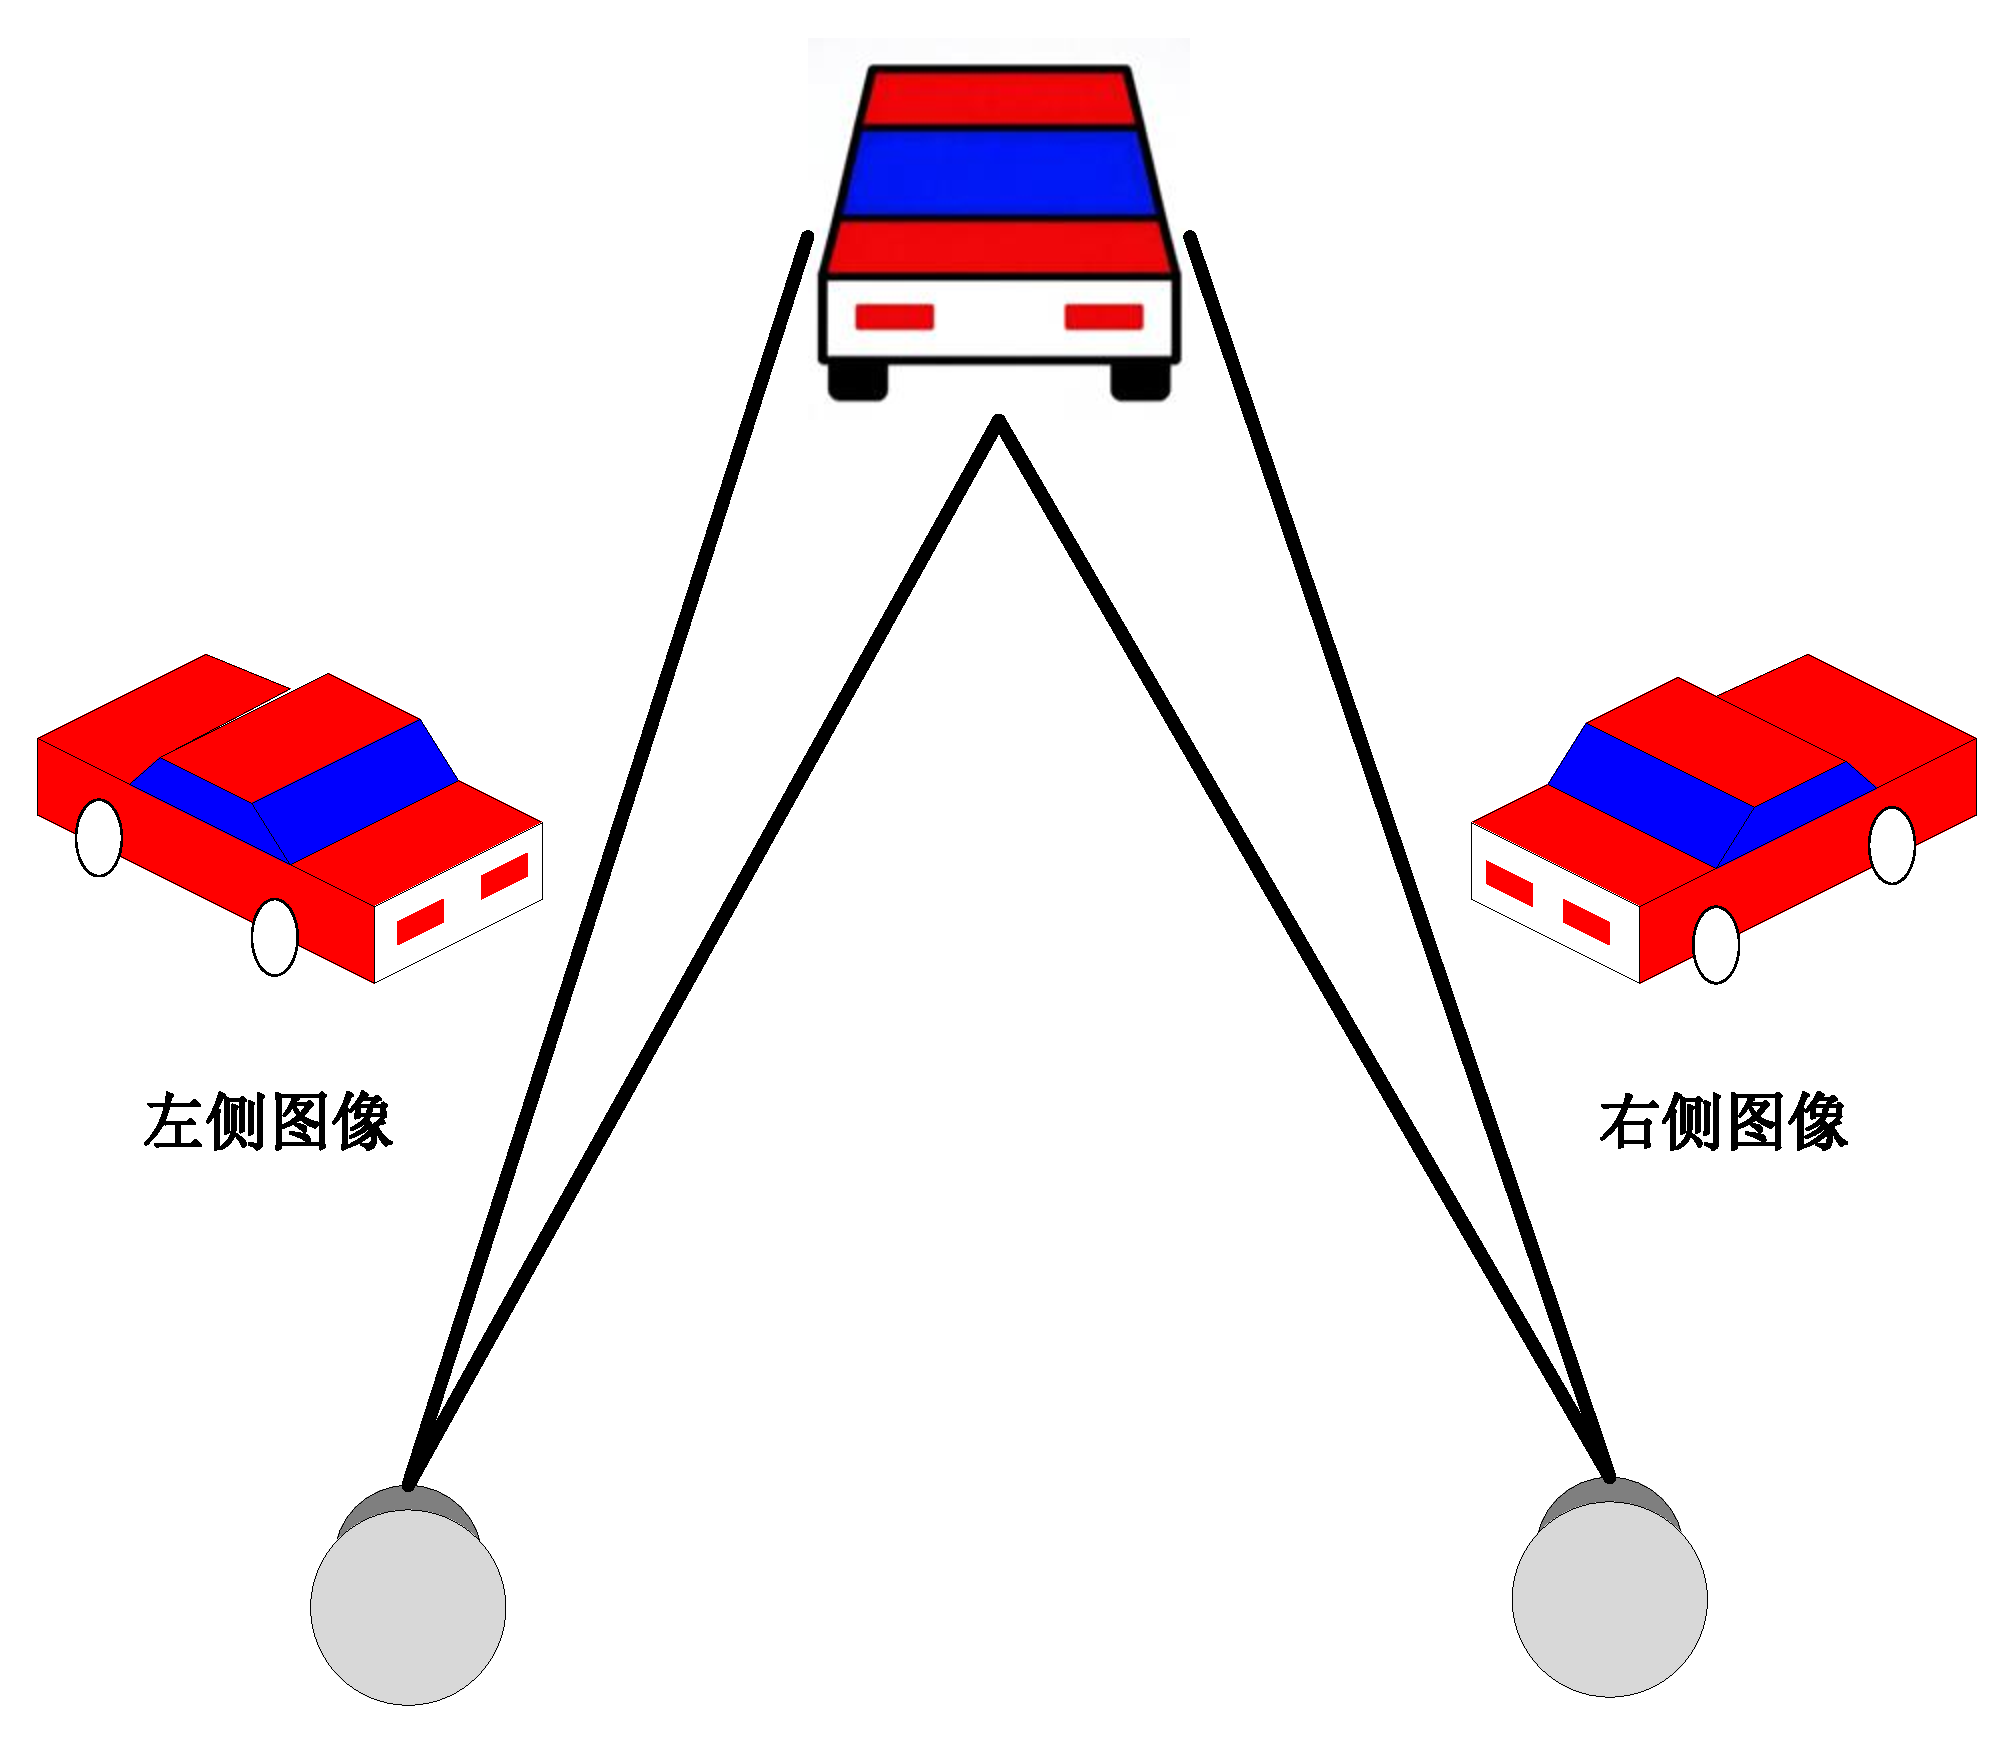
\includegraphics[width=0.9\linewidth, height=4cm]{resources/2p/2-2d.pdf}
    
    \centering\small(d) 
    \label{fig:1-1d}
  \end{minipage}

  \caption{ (a)调节机制示意图 (b)运动视差示意图 (c)辐辏反射示意图 (d)双目视差示意图}  % 替换XXX为子图(d)的说明
  \label{fig:2-2}
\end{figure}



调节机制：如图\ref{fig:2-2}(a)所示，晶状体通过睫状肌改变曲率来完成对焦。不同距离目标对应不同焦距状态，这种动态调节本身就能向大脑提供深度信息\cite{Wandell1995}。

运动视差：当人或相机发生位移时，近景在视野中的运动量明显大于远景（图\ref{fig:2-2}(b)）。这种速度差可稳定揭示物体深度顺序\cite{Ooi2001,Salzman2008}。

辐辏反射：注视近物时双眼会向内汇聚（图\ref{fig:2-2}(c)）。通常辐辏角越大，表示目标越靠近；角度减小则对应更远距离。该线索在中近距离范围内尤为敏感\cite{Schor1987}。在头部轻微运动时，该线索还能与运动视差互补，提高距离判断稳定性。

双目视差：成人瞳距通常处于 60--70 mm 区间，常取约 64 mm。受观察角度差影响，同一目标在左右视网膜上的成像并不重合（图\ref{fig:2-2}(d)），视觉皮层据此恢复深度并建立立体感\cite{Read2002}。

\begin{figure}[htbp]
  \centering
  %\vspace{1 cm} % 使用该指令调整上下间距
  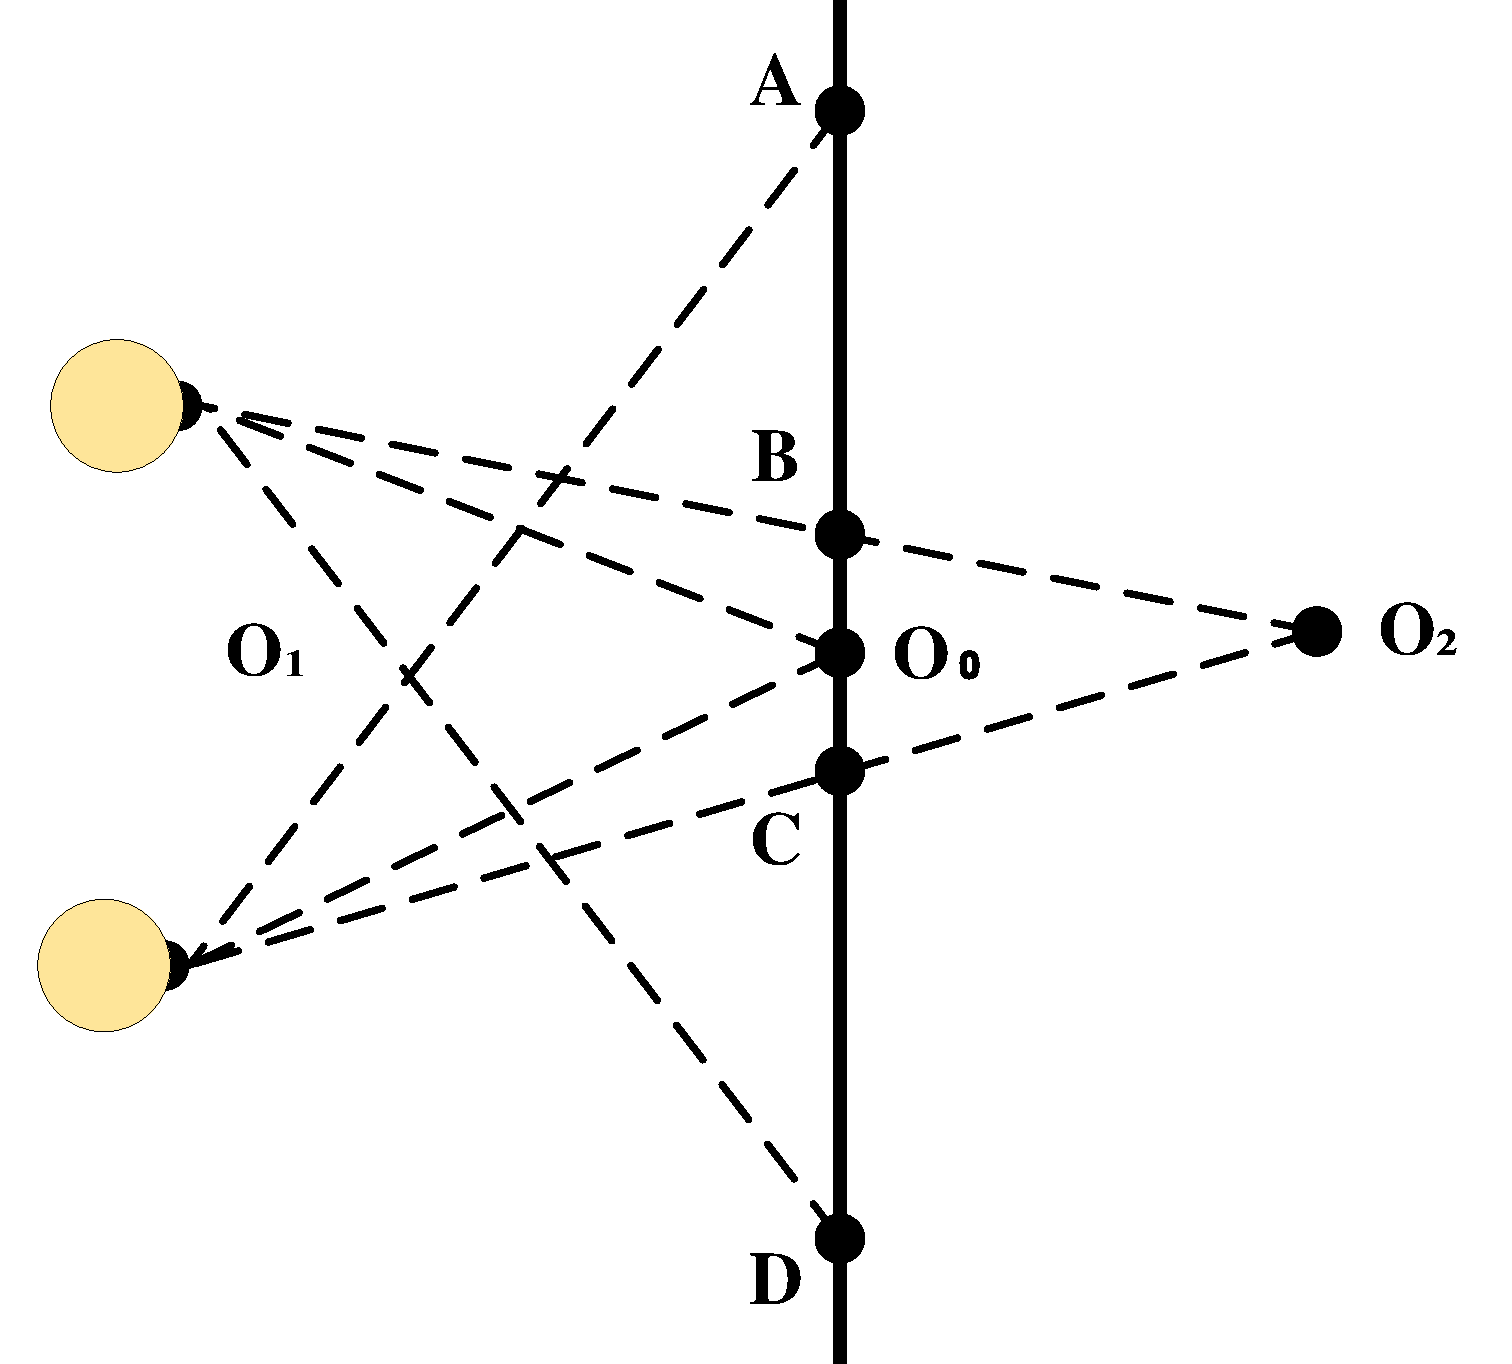
\includegraphics[width=0.5\textwidth]{resources/2p/2-3.pdf}
  % \bicaption{中文标题}{English Caption} % 使用中英文标题
  \caption{显示景深与视差的关系} % 只使用中文标题
  \label{fig:2-3}
  %\vspace{1 cm} % 使用该指令调整上下间距
\end{figure}

图\ref{fig:2-3}给出了景深感知与视差符号的对应关系\cite{Yamamoto2010}：目标位于零视差面时被感知在屏幕平面；当左右眼成像对应 B、C 时，目标 O$_1$ 呈“出屏”效果（正视差）；对应 A、D 时，目标 O$_2$ 呈“入屏”效果（负视差）。据此调节子像素排布和视差量，可在保证舒适性的同时扩展可感知深度范围\cite{Lee2015}。

\subsection{光场显示基础}
除数学定义外，光场模型在工程中还承担“表示接口”的角色：采集系统输出的数据格式、重建网络的输入组织方式以及显示系统的视点编码，通常都依赖同一套参数化约定。换言之，模型选择不仅决定理论表达能力，也直接影响软硬件协同效率。
光场模型用于统一描述空间中全部可见光线及其辐射属性，参数通常包含位置、方向、波长和时间\cite{Levoy2006}。通过该参数化形式，可在采集后进行重建与再渲染。与仅记录颜色强度的二维图像不同，光场数据天然携带角度信息，因此支持后聚焦、视点迁移和遮挡恢复等操作，这些能力对于人脸细粒度光照编辑尤为关键。
1936 年 Gershun 首次提出光场概念\cite{Gershun1936}，1991 年 Adelson 团队进一步给出七维全光函数的形式化表达\cite{Adelson1991}。图\ref{fig:2-4}(a)展示了其参数结构，对应数学式见公式\ref{eq:2-1}：


\begin{equation}
\label{eq:2-1}
I = L(x, y, z; \theta, \varphi, \lambda; t)
\end{equation}

在该表达中，$L$ 表示辐射亮度，$(x,y,z)$ 描述空间位置，$(\theta,\phi)$ 给出方向，$\lambda$ 与 $t$ 分别对应光谱和时间。其物理含义完整，但维度过高，直接用于动态场景采集与重建会显著增加存储与计算负担\cite{Ng2005}。

\begin{figure}[htbp]
  \centering
  % 第一张子图（左侧）
  \begin{minipage}{0.48\textwidth}  % 宽度减半，为左右排列留出空间
    \centering
    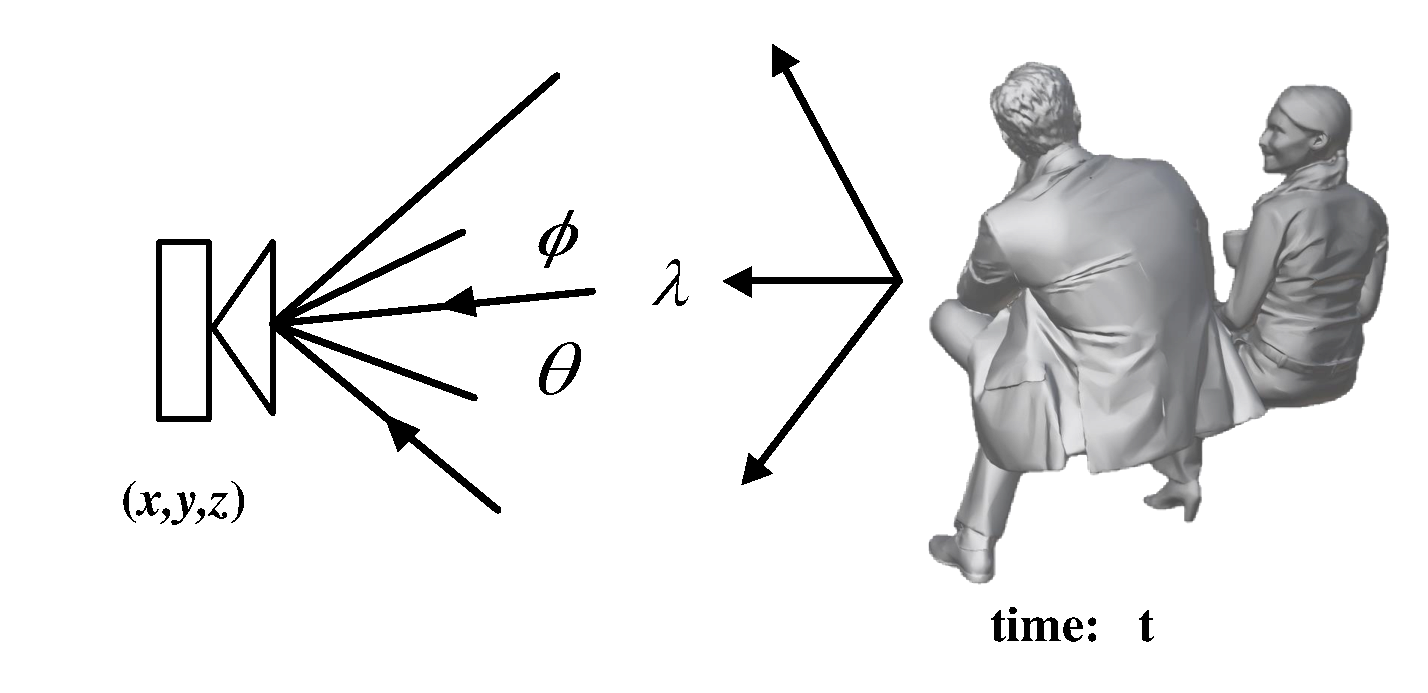
\includegraphics[width=0.9\linewidth, height=4cm]{resources/2p/2-4a.pdf}
    
    \centering\small(a) 
    \label{fig:2-4a}
  \end{minipage}
  \hfill  % 关键：添加水平间距，让两张图左右分开
  % 第二张子图（右侧）
  \begin{minipage}{0.48\textwidth}
    \centering
    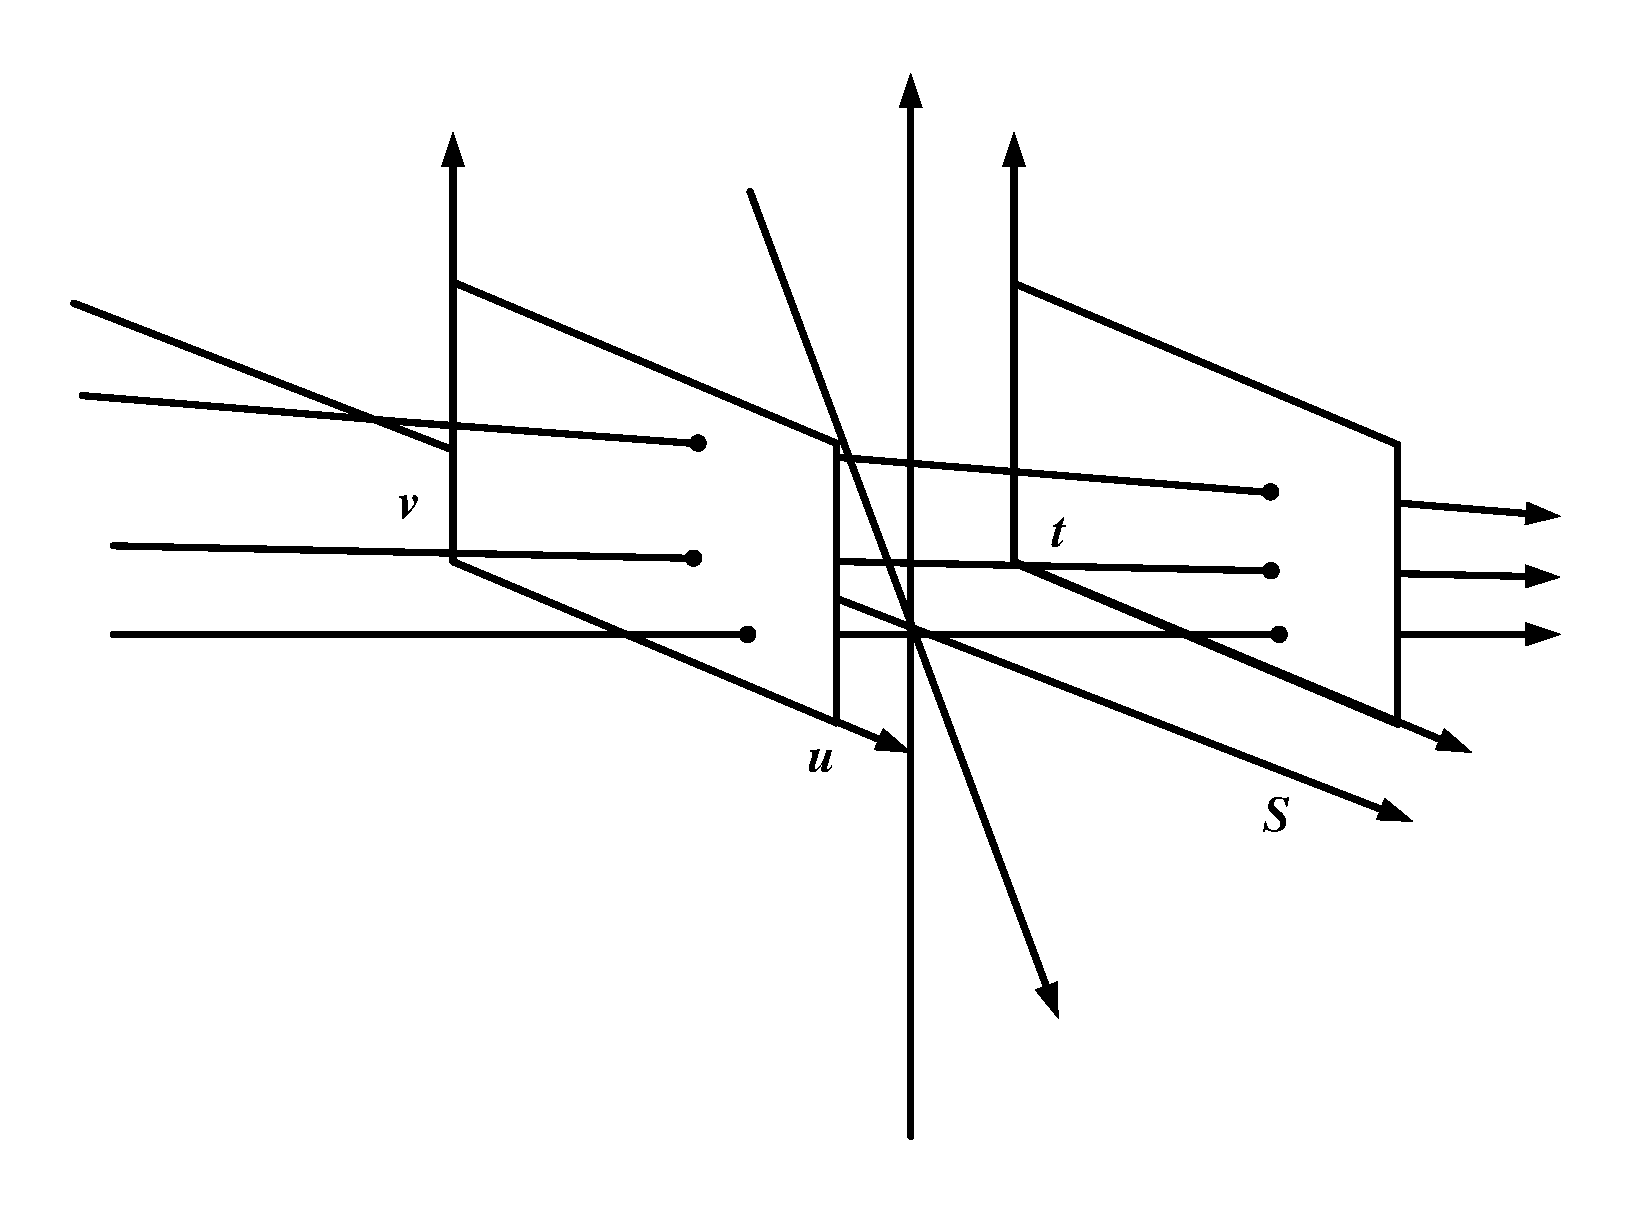
\includegraphics[width=0.9\linewidth, height=4cm]{resources/2p/2-4b.pdf}
    
    \centering\small(b) 
    \label{fig:2-4b}
  \end{minipage}

  % 大图标题：保持不变
  \caption{ (a)七维全光函数数学模型 (b)四维全光函数数学模型}
  \label{fig:2-4}
\end{figure}

为满足工程应用，通常先固定波长与时间维度，将全光函数从七维降至五维。进一步地，Levoy 团队提出双平面参数化（四维光场）\cite{Levoy1996}：用光线与两平行平面 $(s,t)$、$(u,v)$ 的交点唯一表示光线。图\ref{fig:2-4}(b)为其示意，数学形式如\ref{eq:2-2}。
% 独立公式优化版（变量用斜体，保持一致性）
\begin{equation}
\label{eq:2-2}
L = L(s, t, u, v) 
\end{equation}

其中 $(s,t)$ 与 $(u,v)$ 分别对应两平面交点坐标。该表示对少量特殊方向光线的刻画能力有限，但对人眼主要可见光线已足够完整；同时它显著降低了数据规模与重建复杂度，因此成为光场显示与渲染中的主流建模方式\cite{Ng2006}。在实际系统中，四维参数化还能与相机阵列或子孔径图像自然对接，便于后续完成视图插值、深度估计和光照一致性优化。




% 式中：
% \begin{itemize}
%   \item $I$ —— 光场的辐射强度（Intensity）；
%   \item $L$ —— 光场的辐射亮度（Radiance），是光场的核心物理量；
%   \item $(x, y, z)$ —— 三维空间中光线采样点的位置坐标；
%   \item $\theta, \varphi$ —— 光线传播的方位角和俯仰角，表征光线的传播方向；
%   \item $\lambda$ —— 光的光谱波长，决定光的颜色特性；
%   \item $t$ —— 时间维度，用于描述动态光场的变化过程。
% \end{itemize}

\subsection{基于光栅的光场显示器}

在多种光场显示方案中，水平视差柱镜光栅因结构成熟、光利用率高而应用广泛。该技术通过柱面透镜阵列对像素光线进行角度重分配，核心设计变量包括透镜曲率、焦距与排布周期。如图\ref{fig:2-5}(a)(b)所示，LCD 发出的子像素光经柱镜折射后被送往不同观察方向，从而输出多视点图像。与全视差系统相比，水平视差方案牺牲了垂直视差信息，但显著降低视点数量需求，使单视点可获得更高有效分辨率。典型硬件由 LCD、背光、功能膜层和柱镜光栅构成，其中功能膜层可通过调节扩散角提升视点均匀性。

\begin{figure}[htbp]
  \centering
  % 第一张子图（左侧）
  \begin{minipage}{0.48\textwidth}  % 宽度减半，为左右排列留出空间
    \centering
    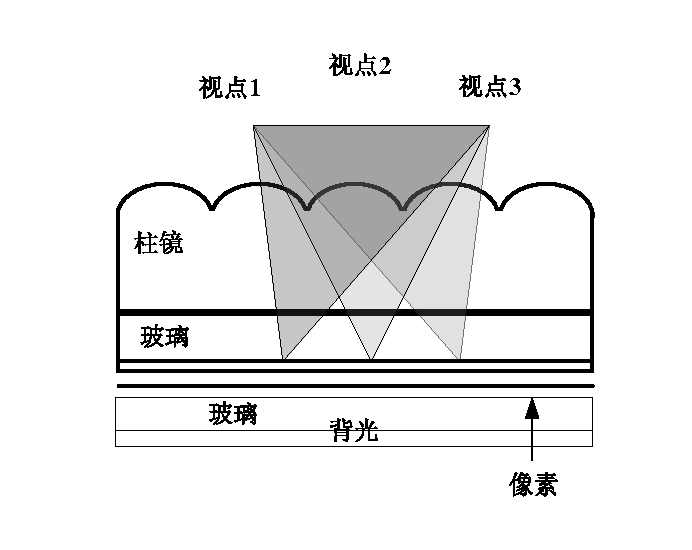
\includegraphics[width=0.9\linewidth, height=6cm]{resources/2p/2-5a.pdf}
    
    \centering\small(a) 
    \label{fig:2-5a}
  \end{minipage}
  \hfill  % 关键：添加水平间距，让两张图左右分开
  % 第二张子图（右侧）
  \begin{minipage}{0.48\textwidth}
    \centering
    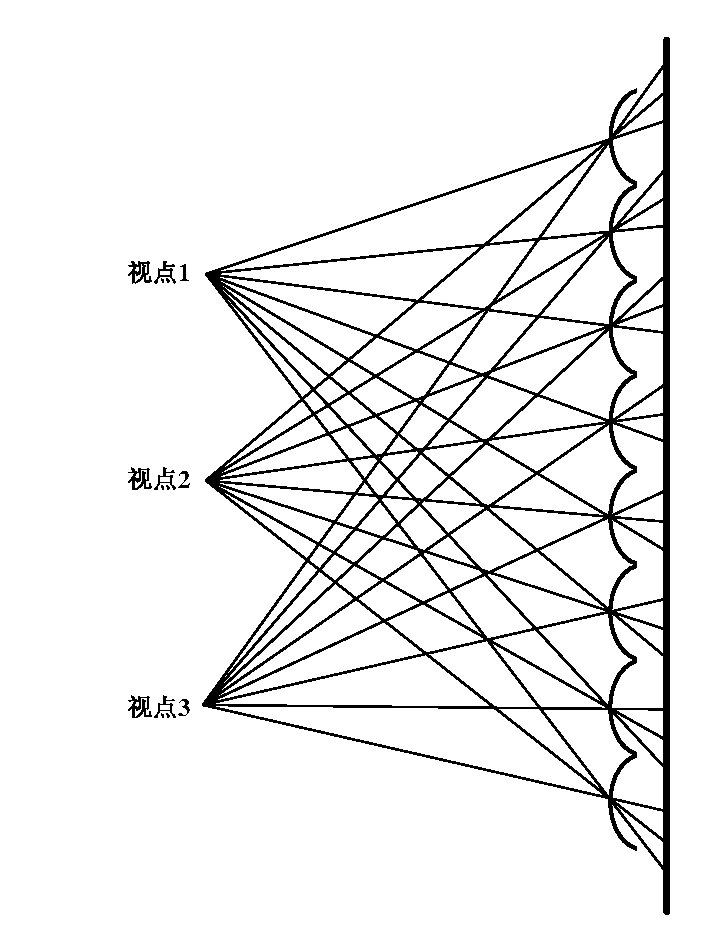
\includegraphics[width=0.9\linewidth, height=6cm]{resources/2p/2-5b.pdf}
    
    \centering\small(b) 
    \label{fig:2-5b}
  \end{minipage}

  % 大图标题：保持不变
  \caption{ (a)柱镜光栅显示器核心组件构成 (b)多视点排列特征及其空间分布规律可视化}
  \label{fig:2-5}
\end{figure}

在具体实现中，显示系统还要兼顾人因约束与硬件约束：人因层面关注观看距离、头部运动范围与视觉舒适阈值，硬件层面关注面板分辨率、透镜加工误差与亮度损失。两类约束共同决定可用视点数量和有效景深窗口。若系统仅追求视点密度而忽略亮度与串扰控制，实际观感反而可能下降。
柱镜的本质作用是把“像素位置”转换成“出射方向”。当 LCD 与柱镜焦面满足共轭关系后，原本发散的子像素光会被重整并沿特定角度传播，使不同像素组分别对应不同视点，实现方向编码。

\begin{figure}[H]
  \centering
  %\vspace{1 cm} % 使用该指令调整上下间距
  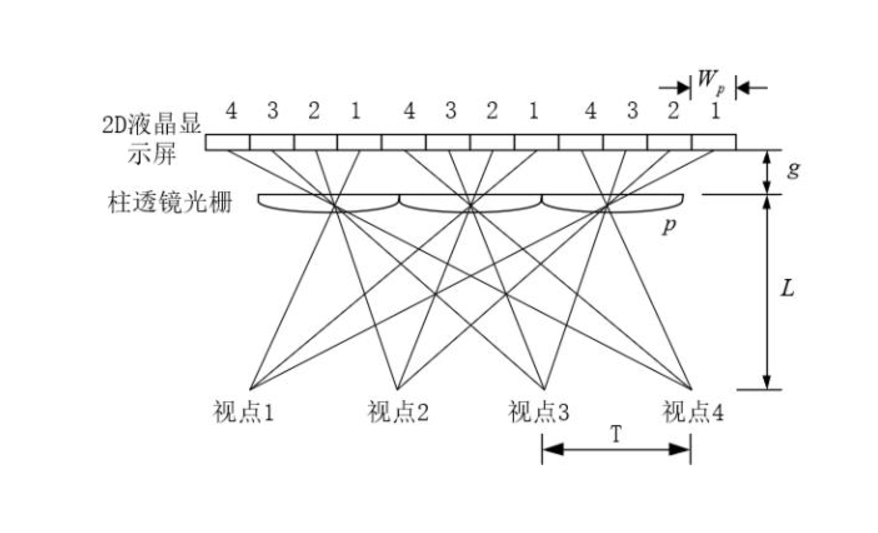
\includegraphics[width=0.8\textwidth,height=6cm]{resources/2p/2-6.pdf}
  % \bicaption{中文标题}{English Caption} % 使用中英文标题
  \caption{柱透镜覆盖子像素原理图} % 只使用中文标题
  \label{fig:2-6}
  %\vspace{1 cm} % 使用该指令调整上下间距
\end{figure}

如图\ref{fig:2-6}所示，当一个柱镜周期覆盖 4 个 LCD 子像素时，系统可形成 $N=4$ 个主视点方向。设计中需要联合优化透镜节距 $p$、曲率半径 $r$、面板间距 $g$、子像素宽度 $W_p$、最佳视距 $L$ 与视点间距 $T$。这些参数满足几何光学关系，可由相似三角推导得到：

\begin{equation}
T = \frac{L}{g} W_p \
\end{equation}

\begin{equation}
\frac{p}{N \cdot W_p} = \frac{L}{g + L} \
\end{equation}

由于柱镜与像素阵列均具周期结构，显示中容易出现摩尔纹和色散伪影。工程实现常将柱镜相对像素栅格倾斜约 $15^\circ$--$20^\circ$（常见取值约 $18^\circ$）以破坏周期共振并抑制干涉纹；再结合像素级或子像素级视点编码，可提升视点过渡连续性与观看稳定性。

\section{三维人脸光照编辑相关物理模型与评价指标}

光场人像编辑并非单一网络即可完成，其效果取决于成像几何、照明表达与渲染求解三部分的协同。为此，本节按“相机模型—光照模型—渲染模型”的顺序展开，分别说明数据从三维空间到二维图像的投影规则、环境光的参数化方式以及外观合成机制，为后续算法设计提供统一物理语境。需要强调的是，三类模型在训练与推理阶段常以“弱耦合、强约束”的方式交互：几何误差会传递到光照估计，光照偏差又会影响渲染一致性，因此评价环节必须同时观察多个维度。

\subsection{相机模型}
相机模型描述了三维点到二维像素的映射链路，如图\ref{fig:2-7}所示：

\begin{figure}[htbp]
  \centering
  %\vspace{1 cm} % 使用该指令调整上下间距
  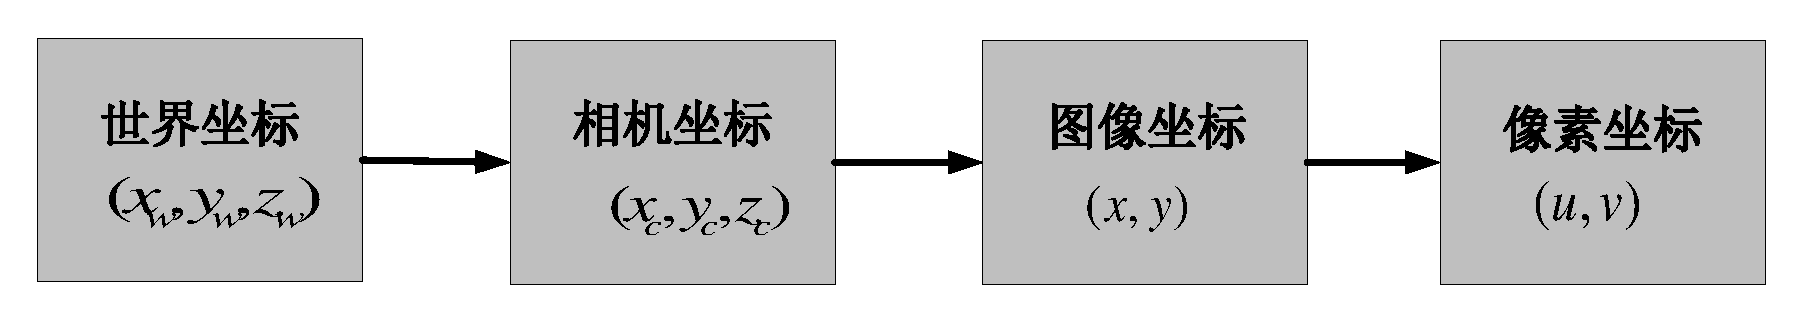
\includegraphics[width=0.8\textwidth,height=2cm]{resources/2p/2-7.pdf}
  % \bicaption{中文标题}{English Caption} % 使用中英文标题
  \caption{物体成像的过程} % 只使用中文标题
  \label{fig:2-7}
  %\vspace{1 cm} % 使用该指令调整上下间距
\end{figure}

相机投影过程可表示为：
\begin{equation}
q = \prod (Rp + t) \
\end{equation}
其中 $R,t$ 组成外参，用于将世界坐标下的点 $p$ 变换到相机坐标系得到 $p'$；符号 $\prod$ 表示投影算子（可对应透视或正交形式），再结合像素采样关系得到最终像素坐标 $q$。

在参数估计实践中，内参与外参通常通过标定板或多视图自标定联合获得。对于人脸视频序列，还需考虑轻微滚动快门、镜头畸变与面部非刚性运动带来的偏差。若这些因素未被建模，投影误差会在训练过程中被网络“错误吸收”，表现为几何漂移或局部纹理拉伸。因此，后续方法中会将基础标定结果与学习式微调结合，以提高整体鲁棒性。

在人脸重建与跟踪任务中，弱透视模型因参数少、求解稳定而常被采用，其表达式为：
\begin{equation}
u = s \cdot (x \cdot f / Z_0 + c_x), \quad v = s \cdot (y \cdot f / Z_0 + c_y) \
\end{equation}
其中 $(x,y,Z_0)$ 为相机坐标系点位，$f$ 为焦距，$Z_0$ 为目标平均深度，$s$ 为整体尺度，$(c_x,c_y)$ 为主点坐标，$(u,v)$ 为输出像素位置。

由于该模型计算代价低，常用于 2D 关键点与稠密配准流程\(^{[85]}\)。对应投影矩阵为：
\begin{equation}
\Pi = s
\begin{pmatrix}
1 & 0 & 0 \\
0 & 1 & 0
\end{pmatrix}
\end{equation}
其中 \(s = 1/d\) 为相似缩放因子，\(d\) 代表平均深度，反映“距离变化导致成像尺度变化”的规律。实际训练时，常将 3D 预测结果投影到 2D，与标注图像比较后构建损失函数。若结合多视图监督，还可额外引入跨视点重投影一致性项，以提升几何稳健性并抑制局部漂移。
\subsection{光照模型}


% 正文内容
光照建模是实现真实感外观的核心难点。传统 Lambert、Phong、Blinn--Phong 等局部模型通常只考虑有限光源，难以完整覆盖环境光、多次反射和间接照明效应\cite{Phong1975,Blinn1977}。随着 HDR 环境贴图与全局照明方法的发展\cite{Debevec1997}，光照表示逐渐转向球面函数框架，即把入射光分布视为单位球面上的连续函数\cite{Ramamoorthi2001}。对于人脸场景而言，这一点尤其重要：皮肤、头发和眼部区域在同一光照下会呈现明显不同的反射特性，低阶模型若表达不足，往往会出现“整体亮度对了但质感失真”的问题。

球谐函数可看作球面傅里叶基，具备正交、完备和良好旋转性质\cite{Morse1953}，因此非常适合低频光照压缩。在实时渲染、PRT\cite{Sloan2002}、三维重建及 NeRF 光照分解等场景中，它已成为基础表示。其定义如下。

在三维欧氏空间中，任一方向向量 $w$ 可通过球坐标表示为：
\begin{equation}  % 替换\[...\]为equation环境，自动编号
w = (\theta, \phi)
\label{eq:2-8}
\end{equation}

其中 $\theta$ 为极角，$\phi$ 为方位角。复数形式球谐函数定义为：
\begin{equation}
Y_l^m(\theta, \phi) = N_l^m P_l^m(\cos \theta) e^{im\phi}
\end{equation}

其中，$l$ 为阶数，$m$ 为次数，$P_l^m$ 为带勒让德多项式，$N_l^m$ 为归一化因子，具体如下：
\begin{equation}
N_l^m = \sqrt{\frac{(2l+1)(l-m)!}{4\pi(l+m)!}}
\end{equation}

在图形学实现中，通常采用实数球谐函数以规避复数运算，实数球谐函数表达式为：
\begin{equation}
Y_l^{m} =
\begin{cases}
\sqrt{2}N_l^{m}\cos(m\phi)P_l^{m}(\cos\theta), & m > 0 \\
N_l^{0}P_l^{0}(\cos\theta), & m = 0 \\
\sqrt{2}N_l^{|m|}\sin(|m|\phi)P_l^{|m|}(\cos\theta), & m < 0
\end{cases}
\end{equation}

通过球谐展开可得到如下表达式：
\begin{equation}
f(w) = \sum_{l=0}^{\infty} \sum_{m=-l}^{l} c_l^m Y_l^m(w)
\end{equation}

其中：
\begin{equation}
c_l^m = \int_{S^2} f(w) Y_l^m(w) dw
\end{equation}

球谐系数可理解为光照在不同角频率上的能量投影：$l=0$ 近似整体亮度，$l=1$ 刻画主照明方向，$l=2$ 主要反映软阴影与低频遮挡；更高阶用于表达高光与锐利阴影。阶数提升会改善细节，但参数量与计算量约按 $O(l^2)$ 增长。

基于球谐函数的光照模型的环境光照表示如下：
\begin{equation}
L(w) \approx \sum_{i=1}^{n} c_i Y_i(w)
\end{equation}

工程实践中常采用三阶 SH（9 个系数）在效率与质量间折中。Lambert 漫反射积分可写为：
\begin{equation}
I(n) = \int_{S^2} L(w) \max(0, n \cdot w) dw
\end{equation}

做球谐卷积近似后可得：
\begin{equation}
I(n) \approx \sum_{i=1}^{9} c_i k_i(n)
\end{equation}

其中 $k_i(n)$ 是与法线方向相关的卷积核项。已有研究表明，Lambert 项通常用二阶 SH 即可达到较好近似精度。

图\ref{fig:2-8}展示了球谐基函数形态。凭借低频表达高效、旋转处理方便等特点，SH 已成为实时渲染与重建系统中的常用组件\cite{Green2003,Kautz2004}；在可微渲染与神经场方法中，它同样被广泛用于光照学习与可编辑表示\cite{Li2020,Martin-Brualla2021}。

\begin{figure}[htbp]
  \centering
  %\vspace{1 cm} % 使用该指令调整上下间距
  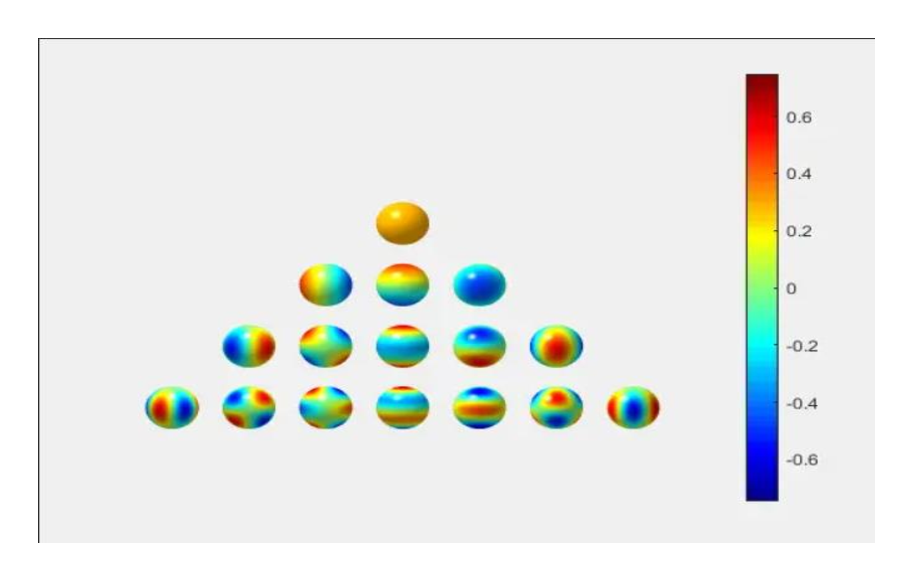
\includegraphics[width=0.8\textwidth,height=8cm]{resources/2p/2-8.pdf}
  % \bicaption{中文标题}{English Caption} % 使用中英文标题
  \caption{球谐函数可视化} % 只使用中文标题
  \label{fig:2-8}
  %\vspace{1 cm} % 使用该指令调整上下间距
\end{figure}

\subsection{渲染模型}
渲染模型在本研究中的作用可概括为“把可估计的物理量转成可感知的视觉结果”。当几何、材质与光照参数发生微小变化时，渲染器需要给出稳定且可解释的像素响应，这一点对光照编辑尤为关键。若渲染过程不稳定，即便网络在训练集上收敛，也容易在跨视角浏览时出现闪烁、明暗漂移或局部伪影。

（1）传统渲染模型
在离线内容生产中，传统渲染管线仍具有不可替代的价值：一方面，材质和灯光参数具备明确物理含义，便于艺术家精细调参；另一方面，成熟的软件生态提供了可靠的资产管理与流程复用能力。对于论文实验而言，传统渲染结果也常被用作对照基准，以评估神经方法在真实感与泛化能力上的增益。

传统渲染模型的核心是依托计算机图形学渲染管线，将三维虚拟几何模型生成具有连续观看效果且真实感较强的三维光场图像。这里的虚拟几何模型通常是人工构建的仿真模型，包含材质和纹理属性。制作者一般使用三维建模软件（如 Blender、3ds Max 等）完成目标建模\cite{BlenderFoundation2019}，在制作阶段通常不直接使用真实场景采集的图像或深度信息。

基于虚拟几何模型的光场内容生成流程通常包括光照模型配置、几何模型布置、纹理与材质映射以及光场编码等环节。早期图形学渲染方法主要依赖光栅化（Rasterization）路径，利用顶点、线段与面片表征虚拟几何模型，并通过纹理映射补充颜色细节。该阶段的光照建模以基础模型为主，例如朗伯光照模型（Lambert's Model）用于刻画漫反射过程，菲涅尔方程（Fresnel equations）用于描述光线在不同介质间的反射和折射\cite{Born1999}。由于难以准确模拟全局光照，早期渲染效果普遍真实性不足。

随着 GPU 计算能力提升与人工建模技术持续优化，基于虚拟几何模型的三维光场内容生成进入新阶段。受益于更高计算效率，面向三维光场的渲染方法在保证一定帧率的同时能够纳入更多提升观看体验的因素，包括更精确的物理渲染机制与更复杂的光照模型以逼近真实场景。在这一背景下，多种可生成更真实光场内容的渲染方法相继提出，并在部分场景实现了实时渲染。

例如，光线追踪技术（Ray Tracing）通过模拟虚拟光线在仿真场景中的传播和虚拟几何模型的交互过程，对光线的反射、折射和阴影等现象进行更为精细的描述\cite{Pharr2016}。基于英伟达的CUDA框架，研究者对投射光线进行并行计算，显著提高了虚拟视点的生成速度，在某些条件下使得基于虚拟几何的三维光场内容生成速度达到了实时。此外，基于蒙特卡洛路径追踪（Monte Carlo Path Tracing）的渲染方法通过对光线的随机采样策略提升了渲染效率。更进一步，基于物理的渲染（Physically Based Rendering, PBR）方法通过双向反射分布函数（Bidirectional Reflectance Distribution Function, BRDF）模拟具有不同材质特性的虚拟几何模型表面特性\cite{Walter2007}。PBR方法统计了不同角度的输入光，在漫反射和高光反射下的光线输出，从而基于物理规律对光线的入射和反射过程进行建模。其反射率方程为：
\begin{equation}
L_o(w_o, x) = \int_{\Omega} f_{brdf}(w_o, w_i, x) \cdot L_i(w_i, x) \cdot (w_i \cdot n) dw_i
\end{equation}

其中，$x$ 表示模型表面被入射光线集中的位置，$w_i$ 表示在半球面范围内入射光线的方向，$w_o$ 为出射光线的方向，$n$ 为模型表面在 $x$ 点的法向量，$L_i$ 是入射光线的辐照度，其包含局部和全局光照，$L_o$ 是出射光线的辐照度。$f_{brdf}$ 为半球面上的BRDF函数，其中包含了对漫反射和高光（镜面）反射的建模，可表示为：
\begin{equation}
f_{brdf} = f_d + f_s = \frac{1 - m}{\pi} \cdot b + \frac{D(h; r, b, m) \cdot F(v, h; b, m) \cdot G(w_i, w_o, h; r)}{(n \cdot w_i) \cdot (n \cdot w_o)}
\end{equation}

其中，$f_d$ 表示漫反射过程，$f_s$ 表示高光反射过程。$m$ 表示金属度，$r$ 表示粗糙度，$b$ 表示基础颜色，$D$ 为法向量项，$F$ 为菲涅尔项，$G$ 为几何项。此外，环境光遮蔽（Ambient Occlusion, AO）的进一步引入能够更加精确地计算出间接光照，同时结合全局光照（Global Illumination, GI）使渲染效果更加贴近真实场景。PBR方法的光照过程不仅考虑了光线在物体表面间的多次光照反射，这使得光照计算不再局限于直接光照，还能够模拟间接光源带来的真实效果。同时，还可基于深度学习对所渲染的画面进行降噪处理。但令人遗憾的是，这种传统渲染模型生成三维光场内容的方式存在很大的不足，比如人工制作的虚拟几何模型本身就缺乏真实物品特有的细节。且在建模的过程中，往往需要依赖复杂的材质及光照设计等手段来弥补渲染过程缺乏的真实感。因此在进行虚拟模型设计及动态模型的制作时往往需要较高的成本。
\subsubsection{基于Nerf的体渲染模型}
神经辐射场技术目前已在三维重建与多视点生成等方向广泛应用，也常被视作新型渲染方法。在利用 NeRF 生成三维光场内容前，需先对目标场景进行稀疏采集，并基于不同视角拍摄的 RGB 图像完成相机内参与外参标定，具体可采用 COLMAP 工具。

\begin{figure}[htbp]
  \centering
  %\vspace{1 cm} % 使用该指令调整上下间距
  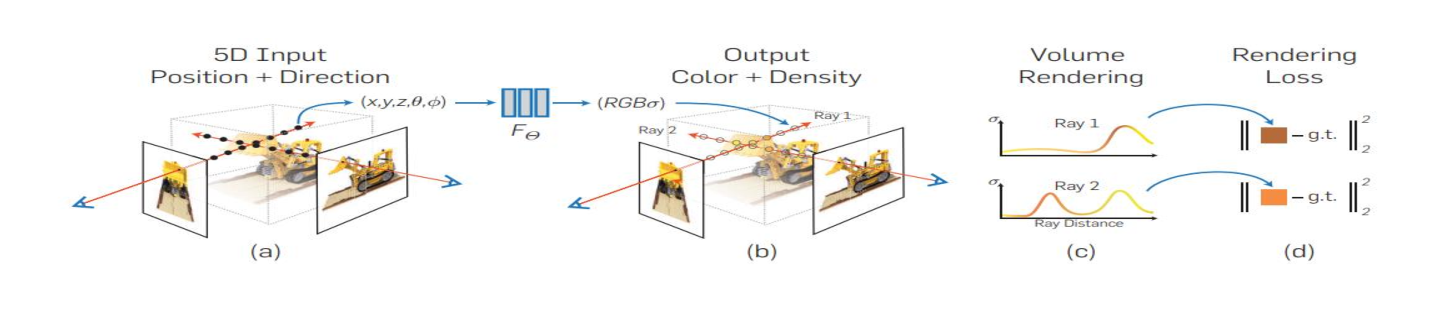
\includegraphics[width=0.9\textwidth,height=4cm]{resources/2p/2-9.pdf}
  % \bicaption{中文标题}{English Caption} % 使用中英文标题
  \caption{Nerf体渲染模型} % 只使用中文标题
  \label{fig:2-9}
  %\vspace{1 cm} % 使用该指令调整上下间距
\end{figure}

NeRF 的整体流程如图\ref{fig:2-9}所示。在训练过程中，NeRF 首先根据求得的相机位姿计算出用于训练的图片中每个像素所对应的渲染光线，其中每条光线可表示为：
\begin{equation}
r(t) = o + td
\end{equation}

其中，$o$ 为对应图像的相机原点，$d$ 为方向向量，$t$ 为光线传播的距离。接下来是第一轮粗采样过程。每个待计算颜色的像素均投射出一根渲染光线并在该光线上进行均匀采样，得到 $N_c$ 个采样点。其中每个采样点 $(x, y, z, \theta, \phi)$ 用其位置 $(x, y, z)$ 和所在射线的方向向量 $(\theta, \phi)$ 共同定义。下一步，NeRF 对输入的采样点进行正余弦位置编码，用于扩充采样点的高频分量，提升神经网络对场景细节的表达能力。其位置编码函数如下：
\begin{equation}
\gamma(p) = \left(\sin(2^0 \pi p), \cos(2^0 \pi p), \dots, \sin(2^{L-1} \pi p), \cos(2^{L-1} \pi p)\right)
\end{equation}

其中 $L$ 为数据扩充的维度参数，对于输入的位置向量，$L$ 的值为 10，对于方向向量，$L$ 的值为 4。之后，将得到的编码向量输入至多层感知机（MLP）神经网络 $F$，用于估计出每个采样点的颜色值和点密度 $\sigma$。其中点密度的估计只与位置向量相关，而颜色值的估计会同时依赖于输入的位置和方向向量。由此可得每个采样点所对应的权重可表示为：
\begin{equation}
w_i = T_i \cdot (1 - \exp(-\sigma_i \delta_i))
\end{equation}

此外，NeRF 使用了重采样策略，根据第一轮粗采样点的位置和权重 $w_i$，通过计算概率密度函数（Probability Density Function, PDF）进行第二轮重要性采样，选取的采样点个数为 $N_f$。之后将第二轮和第一轮的采样点一同输入到第二阶段的神经网络中，预测所有采样点的颜色和点密度值。为了计算图像中每个像素点的颜色，NeRF 方法基于体渲染（Volume Rendering）技术沿着渲染光线传播的方向统计光线上的所有采样点，并用离散化求和的操作来近似连续区域的积分，从而估计每个像素点的颜色。此过程可表示为：
\begin{equation}
\hat{C}(r) = \sum_{i=1}^{N} T_i \cdot (1 - \exp(-\sigma_i \delta_i)) \cdot c_i
\end{equation}

其中，$i \in [1, N]$ 为一条光线上的采样点个数，$\delta_i = t_{i+1} - t_i$ 为第 $i$ 个采样点的线段长度，$c_i$ 为每个采样点的颜色，$T_i$ 表示累积到第 $i$ 个采样点之前的剩余可见度，$\hat{C}$ 为渲染光线所对应的像素颜色。对于优化 NeRF 神经网络的误差函数，NeRF 对预测的颜色 $\hat{C}$ 和对应的真实颜色计算平方误差，定义为：
\begin{equation}
L = \sum_{r \in \mathcal{R}} \left\|\hat{C}(r) - C(r)\right\|_2^2
\end{equation}

网络训练完成后，NeRF 可在目标场景中任意设定观测位置与朝向，从而实现真实场景下的三维光场内容生成。与传统几何驱动方法相比，NeRF 的优势在于对复杂外观细节具有更强拟合能力，尤其在毛发、半透明区域与软阴影边缘等位置表现更稳定；但其代价是训练与渲染开销较大，对数据采集质量也更敏感。因此，实际应用中常结合蒸馏、稀疏采样或网格-神经混合表示来平衡效率与质量。

此外，从系统工程角度看，三维光场人脸光照编辑还涉及数据链路闭环：采集端决定可恢复信息上限，表示端决定可学习结构，显示端决定最终观看体验。若三者在参数定义上不一致，即便单模块性能较高，也可能在端到端流程中出现误差累积。例如，采集时曝光策略与渲染时色彩空间不匹配，会导致光照编辑结果在不同设备上观感差异显著；又如，视点标定存在微小系统误差，可能在视频播放中被放大为轻微抖动。基于此，后续章节的方法设计将尽量采用可解释参数与统一坐标约定，并在训练阶段引入跨视角约束，以降低误差传递风险。
\subsection{图像评价指标}
评价体系不仅用于“给分”，更用于定位问题来源。例如，当 PSNR 提升而 LPIPS 无明显改善时，通常意味着像素误差下降但感知质量收益有限；当 ID 指标下降且 LE/LI 波动增大时，往往提示光照编辑破坏了身份一致性。基于这种诊断逻辑，可更有针对性地调整损失函数权重与训练采样策略。

在实验报告层面，本文也强调“定量结果+可视化现象”的联合呈现。对于光照编辑任务，单纯比较分数可能掩盖一些关键问题，例如高频高光区域局部过曝、边缘区域色偏或跨帧微闪烁等。这些问题不一定显著拉低某个单独指标，却会明显影响主观体验。因此，在后续章节中，除统一给出指标统计外，还会配合典型失败案例分析，说明方法在极端光照与大姿态条件下的行为边界。
为客观评估后续方法在图像质量、跨视角一致性和时间稳定性上的表现，本文构建了多维指标集合：质量指标 FID、PSNR、SSIM、LPIPS；多视角一致性指标 ID、LE、LI；时序指标 WE 与 Temporal LPIPS。各指标定义如下。需要指出，任何单一指标都难以完整反映“可编辑光场人像”的真实质量，因此本文采用组合评价策略：先用像素与感知指标衡量重建准确度，再用身份与时序指标验证编辑稳定性。

此外，在跨数据集比较时还应统一预处理协议，包括人脸对齐、分辨率归一化与掩码区域定义。若这些前处理不一致，指标差异可能主要来自数据管线而非模型本身，导致结论偏差。为避免该问题，本文后续实验将固定评测脚本与随机种子，并在附录给出关键参数。

FID 衡量生成样本分布与真实分布之间的统计距离，是生成任务中常用的感知指标。做法是用预训练 Inception 网络提取两组特征，再计算 Fr'echet 距离：
\begin{equation}
\text{FID} = \left\| \mu_r - \mu_g \right\|_2^2 + \text{Tr}\left( \Sigma_r + \Sigma_g - 2\left( \Sigma_r \Sigma_g \right)^{\frac{1}{2}} \right)
\end{equation}
其中 $\mu_r,\Sigma_r$ 与 $\mu_g,\Sigma_g$ 分别是两组特征的均值和协方差。FID 越小，说明生成分布越接近真实分布。

PSNR 用于刻画像素层面的重建误差，基于均方误差（MSE）定义如下：
\begin{equation}
\text{PSNR} = 10\log_{10} \frac{MAX^2}{MSE}
\end{equation}
其中 $MAX$ 为像素上限（常取 255）。PSNR 越高，表示像素重建误差越小。

SSIM 同时考虑亮度、对比度和结构一致性，表达式为：
\begin{equation}
\text{SSIM}(x, y) = \frac{(2u_x u_y + C_1)(2\sigma_{xy} + C_2)}{(u_x^2 + u_y^2 + C_1)(\sigma_x^2 + \sigma_y^2 + C_2)}
\end{equation}
其中 $u$ 为均值，$\sigma$ 为方差，$\sigma_{xy}$ 为协方差。指标越接近 1，结构相似性越高。

LPIPS 在深度特征空间中比较两幅图像的感知差异，更接近人眼主观判断；数值越小表示视觉上越相似。

ID 指标用于衡量不同视角下人物身份特征的一致性，通常通过人脸识别网络提取嵌入特征向量，并计算余弦相似度：
\begin{equation}
\text{ID} = \frac{f_1 \cdot f_2}{\left\| f_1 \right\| \left\| f_2 \right\|}
\end{equation}

ID 值越高，表示跨视角身份保持越稳定。

LE 衡量相邻帧光照参数或亮度统计的偏移量，值越小说明光照连续性越好。

LI 描述不同视角之间整体光照分布的不一致程度，通常由直方图差或光照方向误差计算，值越低越好。

WE 在光流对齐后计算相邻帧残差，可反映时序几何与纹理稳定性；指标越小越稳定。

Temporal LPIPS 将感知距离扩展到视频域，通过相邻帧特征差异评估闪烁与抖动；数值越低表示时序更平滑。这一点也说明，评价阶段应同时关注“是否逼真”与“是否稳定可控”，二者缺一不可。

从阅读与复现角度出发，本章还尽量统一符号约定和变量含义，减少跨小节理解成本。对同一概念若存在多种称谓，统一采用一次定义、后续复用的写法，以保证全文逻辑闭环。
\section{本章小结}
本章完成了三维光场人脸光照编辑的基础铺垫。首先，从心理与生理两类深度线索解释了立体视觉形成机制，并给出正负视差与景深感之间的对应关系，为后续视差与显示参数设计提供依据。其次，围绕光场建模路径，回顾了从七维全光函数到四维双平面参数化的降维思路，明确了工程可实现性与表达能力之间的平衡点；同时分析了柱镜光栅显示器的结构组成、关键几何参数和抗伪影策略。

在物理建模方面，本章进一步梳理了相机投影、球谐光照、传统 PBR 渲染与 NeRF 体渲染的核心流程，说明了它们在三维人脸外观重建与光照编辑中的功能分工。最后，建立了覆盖图像质量、多视角一致性和时序稳定性的评估指标集合，为后续章节的对比实验与消融分析提供统一度量标准。总体而言，本章给出的理论与模型构成了全文方法设计和实验验证的基础支撑。
为便于后续章节直接继承，本章术语使用尽量保持单义：例如将“光照一致性”限定为跨视角或跨时间的照明参数平稳性，将“身份一致性”限定为人脸语义特征保持，将“结构一致性”限定为几何轮廓与局部纹理关系不失真。这样的定义方式有助于把主观描述转换为可计算目标，避免出现“视觉上更好但无法量化解释”的问题。同时，本章在介绍模型时有意区分了“可解释模型”和“高拟合模型”的角色边界：前者提供可控参数与物理先验，后者负责补足复杂外观细节；二者结合能够在真实感、可控性和泛化性之间取得更稳妥平衡。最后，考虑到论文方法需要面对多设备、多场景与多光照条件，本章所建立的理论框架强调模块可替换性——在不改变整体评价协议的前提下，后续可将不同相机标定策略、不同光照表示或不同渲染后端接入同一流程进行公平比较，这也为后续实验扩展提供了方法学保障。
进一步地，本章也给出了一个可复用的方法学框架：以视觉感知约束定义“看起来自然”，以物理模型约束定义“生成过程合理”，再以多指标评测闭环验证“结果稳定可复现”。该框架既适用于本文任务，也可迁移到其他多视点人像编辑问题。




















